\chapter{Architettura Software dello strumento}
\label{capitolo4}
\thispagestyle{empty}

\textit{In questo Capitolo verrà descritta l'architettura software dello strumento realizzato. Inizialmente verrà analizzato l'ambiente di sviluppo software. Successivamente verrano mostrati i principi alla base della programmazione per microcontrollore e FPGA. Infine, verranno illustrate e descritte le funzionalità implementate su FPGA e microcontrollore.}

\section{Ambiente di sviluppo LabVIEW}
L'ambiente di sviluppo scelto per questo lavoro di Tesi è NI LabVIEW.

LabVIEW, abbreviazione di \textit{Laboratory Virtual Instrumentation Engineering Workbench}, è l'ambiente di sviluppo integrato per il linguaggio di programmazione visuale di \textit{National Instruments}: il linguaggio G (\textit{G-Language}, abbreviazione di \textit{Graphical Language}).

La differenza sostanziale tra il linguaggio G e i linguaggi tradizionali risiede nella sintassi e nel controllo del flusso di programma:
\begin{itemize}
	\item \underline{Sintassi}: La sintassi del linguaggio G non è scritta ma grafica. 
	\item \underline{Controllo del flusso di programma}: Nei linguaggi tradizionali di tipo testuale, l'ordine di esecuzione delle istruzioni che costituiscono il codice del programma è determinato, a meno di ottimizzazioni portate dal compilatore, dall'ordine in cui le istruzioni sono scritte all'interno del codice stesso. Mentre, nel linguaggio G, l'ordine di esecuzione è stabilito dal "flusso di dati", ovvero ciascuna istruzione viene eseguita non appena sono disponibili i suoi dati di ingresso.
\end{itemize}

I programmi generati da LabVIEW prendono il nome di "strumenti virtuali" (\textit{Virtual Instrument}, VI). Un programma VI è composto da due parti fondamentali: il Pannello frontale (\textit{Front Panel}) e il Diagramma a blocchi funzionale (\textit{Block Diagram}).

\begin{figure}
\centering
\subfigure[Front Panel]
{\label{esempiolva}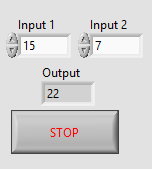
\includegraphics[scale=.8]{cap4/esempiolvaimg}}
\hspace{5mm}
\subfigure[Block Diagram]
{\label{esempiolvb}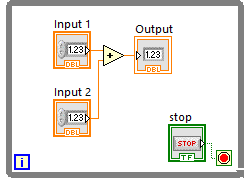
\includegraphics[scale=.8]{cap4/esempiolvbimg}}
\caption{Esempio di LabVIEW VI che calcola la somma di due numeri in virgola mobile}\label{esempiolv}
\end{figure}

Il pannello frontale è l'interfaccia utente del VI. Esso permette di definire ed introdurre tutte le grandezze di ingresso (input del programma) e tutte le grandezze in uscita (valori delle misure, grafici, ecc.). Si realizza con controlli e indicatori, che costituiscono, rispettivamente, i terminali interattivi d'ingresso e d'uscita.
 
Lo schema a blocchi è il diagramma di flusso che rappresenta il codice sorgente, in formato grafico. Esso è composto da due elementi distinti: i \textit{nodi} e i \textit{collegamenti}. I \textit{nodi} sono gli elementi di elaborazione, mentre i \textit{collegamenti} sono i fili che uniscono i vari nodi e permettono lo scambio di informazione ovvero il flusso dei dati.

\begin{figure}  
  \begin{center}
    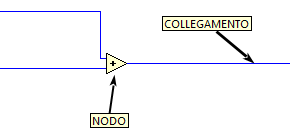
\includegraphics[scale=0.6]{cap4/nodocoll}
    \caption{Esempio di Nodo e di Collegamento}
    \label{nodocoll}
  \end{center}
\end{figure}

Le istruzioni, definite in fase di stesura del codice mediante il linguaggio grafico, vengono tradotte in modo trasparente in linguaggio C e successivamente compilate.

Le caratteristiche principali che hanno portato alla scelta di LabVIEW e del linguaggio G sono:
\begin{itemize}
	\item LabVIEW un ambiente di sviluppo orientato fortemente all'acquisizione dati e all'analisi ed elaborazione numerica di segnali
	\item Il linguaggio G possiede un parallelismo intrinseco che è facile da utilizzare grazie alla metodologia di scrittura grafica dei programmi. La programmazione parallela consente di raggiungere elevate prestazioni di calcolo, specialmente nella programmazione per FPGA
	\item LabVIEW include al suo interno una serie di librerie per l'analisi dei segnali disponibili anche per la compilazione su FPGA che ha notevolmente accelerato il processo di sviluppo del codice
	\item LabVIEW è l'unico linguaggio di programmazione ufficialmente supportato dalla scheda di prototipazione scelta (vedi Capitolo \ref{capitolo3})
\end{itemize}

\section{Sistema Real-Time e FPGA}
Come già accennato nel Capitolo precedente, lo scopo di questo lavoro di Tesi è la realizzazione di un prototipo di un misuratore di distanza basato sull'utilizzo di tecnologie FPGA e microcontrollore.

\subsection{Programmazione del microcontrollore}
	Lo sviluppo di codice per un sistema \textit{embedded} basato su microcontrollore si può suddivere in due approcci:
	\begin{enumerate}
		\item \underline{Bare-metal approach}: consiste in una programmazione a basso livello dove il codice viene caricato direttamente sul dispositivo hardware (in questo caso microontrollore).  Questo approccio è utilizzato quando la complessità del sistema non è elevata. Pertanto garantisce un occupazione di memoria molto piccola (\textit{memory footprint}). Un grosso svantaggio è la poca flessibilità ai cambiamenti di specifiche.
		\item \underline{Real-time Operating System approach}: consiste in una programmazione basata sul supporto di un sistema operativo \textit{Real-Time}. Questo approccio sfrutta tutti i vantaggi dell'utilizzo di un OS (programmazione \textit{multi-thread}, astrazione dell'hardware, ecc...).
	\end{enumerate}
	
	Per i motivi sopracitati si è scelto di sfruttare i vantaggi dell'utilizzo di un sistema Real-Time. Nel paragrafo successivo verrano trattate le caratteristiche dei sistemi Real-Time, i sistemi operativi Real-Time e in particolare il sistema operativo in uso sulla scheda di prototipazione scelta.
	
\begin{figure}  
  \begin{center}
    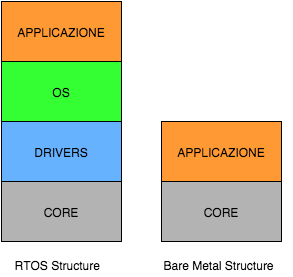
\includegraphics[scale=0.55]{cap4/baremetalrtos}
    \caption{Schema di funzionamento dei due approcci: RTOS e Bare-metal}
  \end{center}
\end{figure}
	
\subsubsection{Sistema Real-Time}

Un \textit{Real-Time System} (RTS) è un sistema in cui la correttezza del comportamento del sistema non dipende solo dall'esattezza dei risultati dei calcoli, ma anche dall'istante temporale in cui questi risultati vengono prodotti \cite{kopetzrt}.

Un'applicazione Real-Time è costituita da un insieme di \textit{task} (compiti) cooperanti. Ogni task possiede una scadenza temporale (\textit{deadline}) entro la quale deve completare la sua esecuzione. Le deadline possono essere di tre tipologie:
\begin{enumerate}
	\item \underline{Hard-deadline}: Una deadline si dice \textit{hard} se le conseguenze della sua violazione portano a un fallimento del sistema.
	\item \underline{Firm-deadline}: Una deadline si dice \textit{firm} se i risultati del corrispondente \textit{task} cessano di essere utili non appena la scadenza viene violata \cite{259423}. Gli effetti della sua violazione non sono catastrofici ma degradano le prestazioni del sistema.
	\item \underline{Soft-deadline}: Una deadline si dice \textit{soft} se l'utilità dei risultati prodotti dal task diminuiscono nel tempo dopo la scadenza. Gli effetti della sua violazione non produce problemi.
\end{enumerate}

\paragraph{Sistema Operativo Real-Time}
Un sistema operativo real-time (abbreviato RTOS, \textit{Real-Time Operating System}) è un sistema operativo specializzato al supporto di applicazioni Real-Time.

Gli RTOS sono solo un elemento di un più complesso sistema real-time. I loro obiettivi sono quelli di fornire un ambiente comodo per riuscire a sviluppare efficacemente l'applicazione gestendo al meglio le risorse, ma soprattutto rispettando i vincoli temporali imposti \cite{fornacia}.

Gli aspetti principali che differenziano un RTOS rispetto a un normale sistema operativo sono:
\begin{itemize}
	\item \underline{Determinismo}: è in grado di svolgere operazioni entro limiti di tempo prefissati.
	\item \underline{Latenza}: La latenza è l'intervallo di tempo che intercorre fra il momento in cui arriva l'input al sistema ed il momento in cui è disponibile il suo output. Nei RTOS viene posto un limite massimo al tempo di latenza per garantire il determinismo.
	\item \underline{Controllo utente}: Il controllo utente è più ampio rispetto ai normali OS. Il programmatore ha un controllo più fine sulle priorità, sull'uso di memoria dei processi e sulla gestione degli interrupt.
	\item \underline{Affidabilità}: Gli RTOS sono progettati in modo da far fronte ai fallimenti del sistema, cercando di preservare quante più informazioni possibili. Contrariamente ai normali OS, non si notifica solo il guasto all'utente ma si cerca di risolvere il problema.
\end{itemize}

Lo scheduling nei RTOS è solitamente semplificato: politiche FIFO o \textit{Round-Robin}. \'E comune l'utilizzo della prelazione (\textit{preemption}) e delle priorità.

I Sistemi Operativi Real-Time più comuni in commercio sono: \textit{VxWorks}, \textit{LynkOS} e \textit{Windows CE}. Esistono anche RTOS gratuiti e \textit{open-source} come: \textit{FreeRTOS} e \textit{eCos}.

L'RTOS presente sulla scheda di prototipazione utilizzata è \textit{VxWorks}.


\subparagraph{VxWorks}
\textit{VxWorks}, prodotto da \textit{WindRiver}, è il più famoso sistema operativo per applicazioni real-time; la notorietà è dovuta al suo utilizzo da parte della NASA nelle sonde spaziali \cite{fornacia}.

La struttura del sistema operativo è basata su \textit{micro-kernel}. Il \textit{micro-kernel}, contrariamente al kernel monolitico, fornisce solo le funzionalità strettamente necessarie alla gestione dei processi. Le funzionalità accessorie, come ad esempio la gestione di rete, sono rese disponibili da librerie esterne al kernel. Questa soluzione offre un ristretto utilizzo di memoria e libertà al progettista di personalizzare il sistema con le funzionalità prescelte.

\begin{figure}  
  \begin{center}
    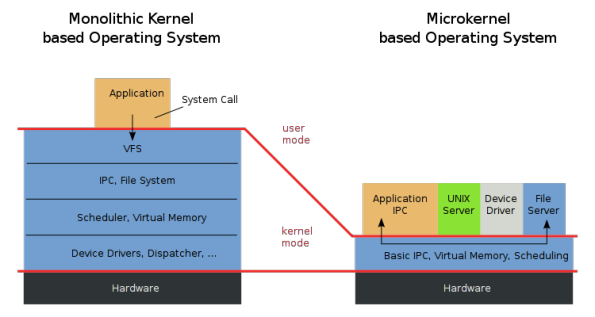
\includegraphics[scale=0.5]{cap4/microvsmono}
    \caption{Confronto tra kernel monolitico e micro-kernel}
  \end{center}
\end{figure}

Lo scheduling utilizzato da \textit{VxWorks} utilizza la politica Round-Robin con diritto di prelazione e priorità. I task con priorità più elevata vengono eseguiti per primi e nel caso di task con la stessa priorità l'esecuzione è Round-Robin.
\begin{figure}  
  \begin{center}
    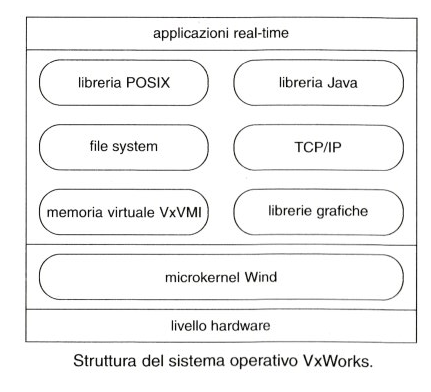
\includegraphics[scale=0.5]{cap4/vxworks}
    \caption{Struttura del sistema operativo VxWorks}
  \end{center}
\end{figure}

La comunicazione tra processi può sfruttare una serie di meccanismi predefiniti come: strutture dati condivisibili (es. variabili globali), semafori e code.

Maggiori informazioni sul sistema operativo \textit{VxWorks} si possono trovare sul sito web dello sviluppatore \cite{sitevxworks}.

\paragraph{LabVIEW Real-Time}
Per lo sviluppo dell'architettura Real-Time di questo lavoro di Tesi è stato utilizzato il modulo software LabVIEW Real-Time.

NI LabVIEW \textit{Real-Time Module} è un componente aggiuntivo di LabVIEW utilizzato per la creazione di applicazioni Real-Time in esecuzione su dispositivi hardware \textit{embedded}.

\begin{figure}  
  \begin{center}
    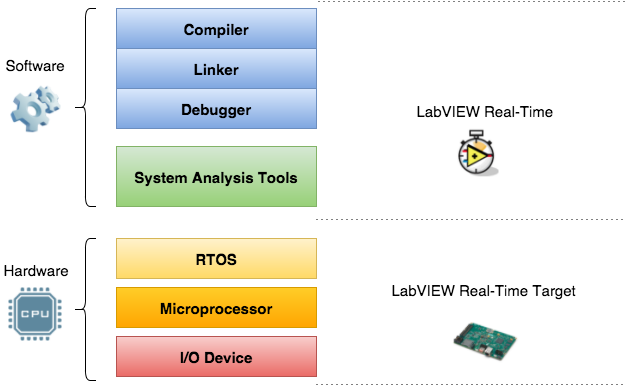
\includegraphics[scale=0.5]{cap4/lvrt}
    \caption{Struttura del modulo LabVIEW Real-Time}
    \label{labviewrt}
  \end{center}
\end{figure}

\begin{figure}  
  \begin{center}
    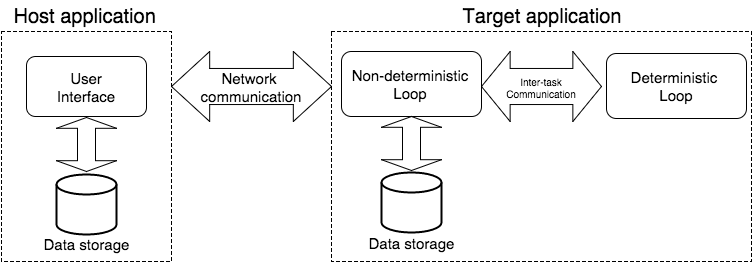
\includegraphics[scale=0.4]{cap4/lvrtvi}
    \caption{Architettura software di un applicazione LabVIEW Real-Time}
    \label{labviewrtvi}
  \end{center}
\end{figure}

La Figura \ref{labviewrtvi} mostra l'architettura software di base di un'applicazione Real-Time sviluppata in LabVIEW. Un applicazione LabVIEW Real-Time si divide in due parti: applicazione \textit{host} e \textit{target}.

L'applicazione \textit{host}, eseguita sul computer host, ha il compito di interfacciarsi con l'utente e comunicare con l'applicazione target. 

L'applicazione \textit{target}, invece, è l'applicazione Real-Time eseguita dal microprocessore del target computer. Nel nostro lavoro di Tesi il target computer è la scheda di prototipazione \textit{Single Board RIO 9636} ampiamente descritta nel Capitolo \ref{capitolo3}.

L'applicazione \textit{target} è composta da processi. Un processo è un insieme di operazioni che si ripetono iterativamente nel tempo consumando una precisa quantità di tempo del microprocessore (\textit{deadline}).
\begin{figure}
\centering
\subfigure[Timed Loop (Deterministico)]
{\label{timedloop}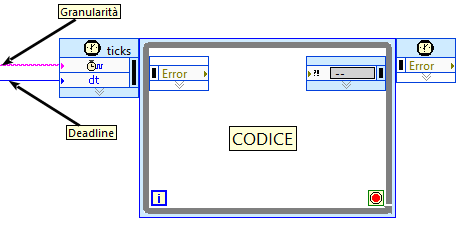
\includegraphics[scale=.5]{cap4/timed}}
\hspace{5mm}
\subfigure[While Loop (Non deterministico)]
{\label{whileloop}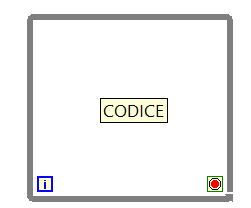
\includegraphics[scale=.5]{cap4/while}}
\caption{Cicli deterministici e non-deterministici}
\end{figure}

In LabVIEW un processo è rappresentato graficamente da un ciclo (\textit{loop}) in cui sono racchiuse le operazioni da eseguire. Essi si suddividono in due categorie:
\begin{enumerate}
	\item \underline{Deterministici} (\textit{Deterministic loop/process}): processi \textit{Hard-deadline}. Sono rappresentati graficamente da Timed Loop (Figura \ref{timedloop}).
	\item \underline{Non Deterministici} (\textit{Non-deterministc loop/process}): processi \textit{Soft-deadline}. Sono rappresentati graficamente da While Loop (Figura \ref{whileloop}).
\end{enumerate}

\subsection{Programmazione dell'FPGA}
FPGA, ampiamente descritto nel Capitolo \ref{capitolo3}, è un dispositivo logico le cui funzionalità sono programmabili via software.

Una delle tecniche più utilizzate per specificare la funzionalità di un dispositivo logico riprogrammabile consiste nell'uso di un linguaggio di descrizione dell'hardware (HDL, \textit{Hardware Description Language}). Esistono anche tecniche che utilizzano strumenti grafici (EDA, \textit{Electronic Design Automation}) per definire lo schema circuitale.

L'HDL è adatto alla progettazione di grandi architetture perché permette di definire numericamente gli elementi circuitali. Tuttavia, l'utilizzo dello schema circuitale permette una lettura dell'architettura più chiara rispetto all'HDL.

\subsubsection{Linguaggi di descrizione dell'Hardware (HDL)}
Un linguaggio per la descrizione dell'hardware o HDL (\textit{Hardware Description Language}) è uno strumento di supporto alla progettazione dei circuiti digitali che ha lo scopo di cogliere gli aspetti funzionali e architetturali di un sistema \cite{fornacia}.

La principale caratteristica di un HDL è la concorrenzialità: ovvero le diverse parti di un codice HDL una volta tradotte in un circuito elettronico, funzionano contemporaneamente, in quanto dispongono di hardware dedicato; al contrario, di un linguaggio software.

Esistono due linguaggi di descrizione dell'hardware attualmente utilizzati: VHDL e Verilog. La toolchain utilizzata per lo sviluppo di questo progetto, che verrà descritta in seguito, fa uso del linguaggio VHDL.

\paragraph{VHDL}
VHDL è l'acronimo di \textit{VHSIC Hardware Description Language}, dove VHSIC è un altro acronimo: \textit{Very High-Speed Integrated Circuits} \cite{storeyelet}.

La metodologia di programmazione di questo linguaggio si basa sul concetto di componente. Il componente è un'unità funzionale e il sistema è rappresentato da una rete gerarchica di componenti.

Le principali fasi di progettazione sono due:
\begin{itemize}
	\item \underline{Entity}: Un entity definisce l'interfaccia di un componente, in particolare le porte di comunicazione e altri parametri come: tempi di ritardo, larghezza del bus, ecc.
	\item \underline{Architecture}: L'architecture definisce la funzionalità svolta dal componente. Per questa fase vengono usati di solito due stili:
	\begin{enumerate}
		\item \underline{Behavioural}: La relazione funzionale ingressi-uscite è espressa tramite un algoritmo. Vengono utilizzati i costrutti noti dei linguaggi di programmazione software come \textit{if-then-else}.
		\item \underline{Structural}: Non viene evidenziata la funzionalità ma la struttura interna del componente. La struttura è formata da componenti di basso livello (segnali, elementi di memoria, ecc.) ed i loro collegamenti (RTL, \textit{Register Transfer Level}).
	\end{enumerate} 
\end{itemize}

VHDL è diventato lo standard IEEE $1076$ nel $1987$. \'E stato aggiornato nel $1993$ ed è conosciuto oggi come "standard IEEE $1076$ $1993$" \cite{545676}. 
		
\subsubsection{Sintesi Hardware}
La sintesi Hardware è il processo di compilazione che trasforma una specifica hardware, espressa in HDL o con schema circuitale, in un file di configurazione per il dispositivo hardware riprogrammabile.

Le principali fasi della sintesi hardware sono:
\begin{itemize}
	\item \underline{Translation}: Molti software per la sintesi hardware consentono al programmatore di poter scrivere la specifica hardware in diversi modi (HDL o schema circuitale). La prima fase della compilazione consiste nel combinare e tradurre le diverse specifiche in un'unica specifica completa.
	\item \underline{Functional simulation}: Questa fase consiste nella simulazione dell'architettura progettata. Questo processo verifica la correttezza logica del circuito senza considerare i vincoli temporali.
	\item \underline{Optimisation}: Dopo che l'architettura è stata valutata logicamente corretta, viene effettuata un ottimizzazione automatica al fine di semplificarne l'implementazione. Le ottimizzazioni più comuni sono le semplificazioni aritmetico-logiche.
	\item \underline{Mapping}: L'architettura ottimizzata viene distribuita sulle risorse disponibili del dispositivo hardware. Il processo è molto impegnativo nel caso di programmazione FPGA perché esistono svariati modi per tracciare le interconnessioni.
	\item \underline{Place and route}: La configurazione risultante dal processo di Mapping viene sottoposta ad una dettagliata simulazione temporale. Questa fase verifica che l'architettura realizzata rispetti i vincoli temporali sul dispositivo hardware reale.
	\item \underline{Configuration data}: Se i risultati della simulazione temporale sono soddisfacenti, viene generato un file di configurazione chiamato \textit{bitfile}. Il \textit{bitfile} contiene tutte le informazioni necessarie per configurare correttamente l'architettura progettata sul dispositivo hardware programmabile.
\end{itemize}

\begin{figure}  
  \begin{center}
    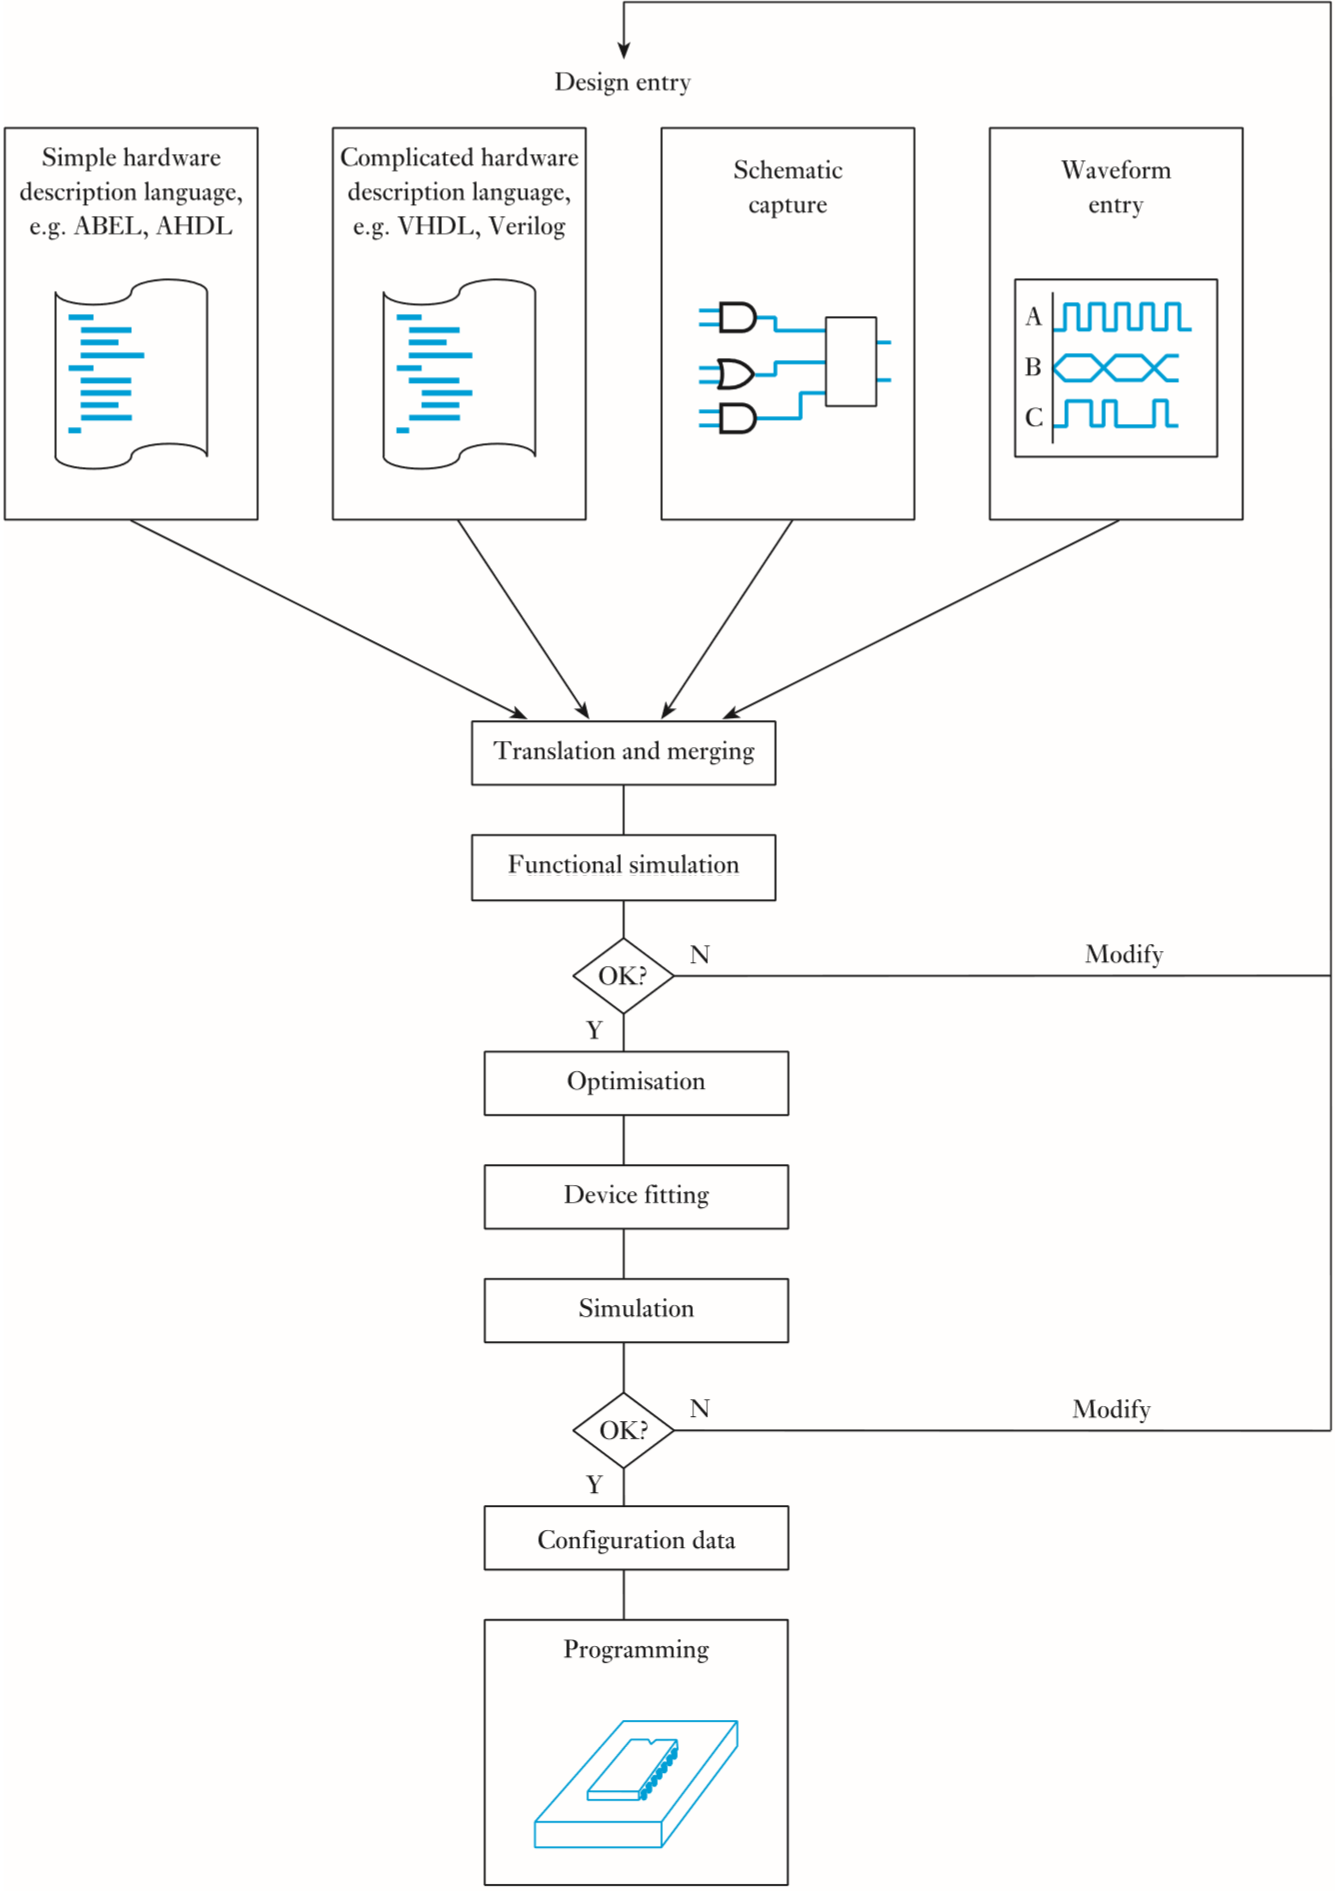
\includegraphics[scale=0.35]{cap4/sinthw}
    \caption{Sintesi hardware}
  \end{center}
\end{figure}
		
\subsubsection{High-Level Synthesis (HLS)}
\textit{High-level synthesis} (HLS), in italiano Sintesi ad alto livello, è un processo automatizzato di compilazione che interpreta una descrizione algoritmica di un desiderato comportamento e crea l'hardware digitale che implementa tale comportamento \cite{Coussy:2008:HSA:1457713}.

La descrizione algoritmica del comportamento è espressa con linguaggi di alto livello come C, infatti è talvolta chiamata \textit{C-Synthesis}. Nella pratica, gli strumenti di compilazione HLS convertono codice C o C-like in un linguaggio di descrizione dell'hardware (HDL), come VHDL o Verilog. 

La scrittura di codice di alto livello permette al progettista di concentrarsi solo sull'aspetto funzionale dell'architettura. Quindi, ad un livello di astrazione più alto, sono necessari meno dettagli per la descrizione di un comportamento. Ad esempio, non si ha bisogno di preoccuparsi dei dettagli implementativi come gerarchie, processi, temporizzazioni, ecc.. come avviene per i linguaggi di descrizione dell'hardware. Questo rende la descrizione molto più facile da scrivere, riducendo notevolmente il rischio di errori e il tempo di testing. 

La sintesi HLS è costituita da una serie di attività e diversi tool HLS eseguono queste attività in ordine diverso utilizzando algoritmi differenti. Altri tool HLS combinano alcune di queste attività e le eseguono iterativamente al fine di convergere verso la soluzione desiderata \cite{eetimes}.

Di seguito vengono elencati i passi principali del processo di sintesi di alto livello:
\begin{enumerate}
	\item \underline{Algorithm optimization}: Nella prima fase, vengono eseguite ottimizzazioni del codice comunemente usate nei compilatori dei linguaggi ad alto livello come ad esempio: \textit{Common Subexpression Elimination} (CSE), \textit{Constant Propagation}, ecc.
	\item \underline{DataFlow Graph analysis}: Vengono analizzate le operazioni aritmetico-logiche e le dipendenze tra i dati. Il risultato di questa analisi si traduce nella costruzione di un grafo chiamato \textit{DataFlow Graph} (DFG). Il grafo rappresenta le dipendenze dei dati e indica l'ordine di esecuzione delle operazioni.
	\item \underline{Resource allocation}: Dopo che il DFG è stato creato, ogni operazione aritmetico-logica viene attribuita ad una risorsa hardware. La risorsa hardware corrisponde ad un'implementazione fisica dell'operatore aritmetico-logico. Ogni operatore può avere più implementazioni hardware, ciascuna con differenti caratteristiche di area/ritardo/latenza. Queste risorse sono selezionate da una libreria tecnologica che contiene tutte le implementazioni disponibili.
	\item \underline{Scheduling}: Questa fase introduce il concetto di tempo e di parallelismo. Lo scheduling prende le operazioni descritte nel DFG e decide quando (in quale ciclo di clock) saranno eseguite \cite{bluebook}.
	\item \underline{Module binding}: Il module binding è la fase che assegna le operazioni aritmetico-logico a specifiche istanze di risorse hardware. Questa fase si basa sulle tipologie e le quantità di risorse hardware scelte nella fase di resource allocation.
	\item \underline{Register binding}: I registri di memoria sono necessari quando i valori prodotti in un ciclo di clock vengono utilizzati in un ciclo di clock differente. La fase del Register Binding consiste nell'allocare i registri necessari a conservare questi valori. In questa fase viene effettuata l'analisi del ciclo di vita di ogni valore allo scopo di poter utilizzare lo stesso registro fisico per memorizzare valori diversi in istanti di tempo diversi.
	\item \underline{Output processing}: I risultati prodotti dai passi precedenti vengono tradotti in codice HDL.
\end{enumerate}

Per i motivi esposti all'inizio del paragrafo, abbiamo scelto di utilizzare un'ambiente di sviluppo che permettesse di sfruttare i benefici della sintesi ad alto livello. L'ambiente di sviluppo utilizzato per la programmazione della scheda FPGA è descritto nel paragrafo successivo.

\begin{figure}  
  \begin{center}
    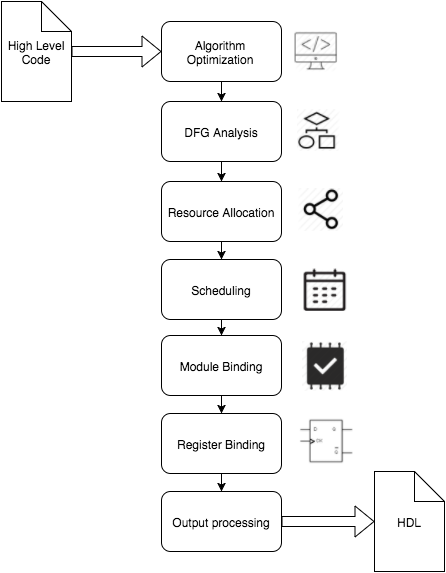
\includegraphics[scale=0.4]{cap4/hls}
    \caption{High Level Synthesis}
  \end{center}
\end{figure}
		
\subsubsection{LabVIEW FPGA}
Per lo sviluppo dell'architettura FPGA di questo lavoro di Tesi è stato utilizzato il modulo software LabVIEW FPGA. NI LabVIEW \textit{FPGA Module} è un componente aggiuntivo di LabVIEW utilizzato per sviluppare applicazioni per FPGA.

Questo ambiente di sviluppo compila ed esegue il codice LabVIEW sul dispositivo FPGA. Il processo di compilazione automatica è suddiviso in tre fasi:
\begin{enumerate}
	\item \underline{High-Level Synthesis}: Il codice di alto livello LabVIEW viene tradotto in codice VHDL
	\item \underline{Hardware Synthesis}: Il codice VHDL, prodotto nel passo precedente, viene tradotto dal compilatore \textit{Xilinx ISE}. \textit{Xilinx ISE Compiler} è uno strumento software prodotto da \textit{Xilinx} che effettua la sintesi hardware di codice HDL. Il risultato finale di questa fase è l'FPGA \textit{bitfile}.
	\item \underline{Bitfile download}: Il \textit{bitfile} generato dal compilatore di \textit{Xilinx} viene caricato ed eseguito sull'FPGA.
\end{enumerate}

\begin{figure}  
  \begin{center}
    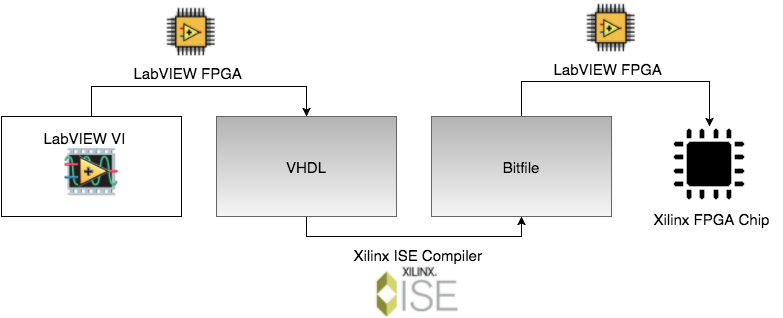
\includegraphics[scale=0.4]{cap4/fpgalv}
    \caption{Processo di compilazione LabVIEW FPGA}
  \end{center}
\end{figure}

Al contrario del microprocessore, non esiste alcun sistema operativo sul chip FPGA, ma LabVIEW FPGA offre comunque la possibilità di controllare ingressi e uscite attraverso un applicazione host.

%% TODO Cap4 Controllare formule analisi teorica algortimi	
\section{Analisi teorica degli algoritmi implementati}
In questo paragrafo verranno introdotti i concetti fondamentali alla base dei principali algoritmi utilizzati nell'ambito dello sviluppo del firmware dell'interferometro.

Gli algoritmi utilizzati sono:
\begin{itemize}
	\item Fast Fourier Transform (FFT)
	\item Interpolated Fast Fourier Transform (IFFT)
	\item Calcolo della distanza assoluta
\end{itemize}

\subsection{Fast Fourier Transform (FFT)}
Prima di illustrare il funzionamento dell'algoritmo di FFT, è bene richiamare alcuni concetti sull'analisi in frequenza dei segnali.

I principali metodi di analisi dei segnali di misura sono l'analisi nel dominio del tempo e nel dominio della frequenza. I due approcci sono tra loro intercambiabili, ovvero, sotto opportune condizioni, nessun informazione viene persa nel passare da un dominio all'altro. 

Lo strumento matematico che consente di trasferire lo studio dei segnali dal dominio del tempo al dominio della frequenza è la trasformata di \textit{Fourier}.

Il campionamento di un segnale analogico $x(t)$ consiste nel prenderne solo i valori $x(iT_s)$ in corrispondenza di istanti ben precisi $iT_s$ detti istanti di campionamento. 
Il campionamento ideale consiste nel moltiplicare il segnale $x(t)$ per il treno di impulsi $s(t)$:
\begin{equation}
	x_s(t)=x(t) s(t) = \sum_{n=-\infty}^{+\infty} x(nT_s) (\delta (t-nT_s))
\end{equation}
\begin{figure}  
  \begin{center}
    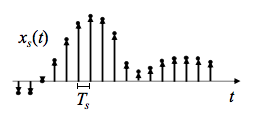
\includegraphics[scale=0.6]{cap4/trenoimp}
    \caption{Segnale campionato con treno di impulsi}
  \end{center}
\end{figure}

Lo spettro in frequenza del segnale campionato è dato dalla Trasformata di Fourier Tempo Discreta (DTFT), espressa dall'equazione: 
\begin{equation}
	X(e^{j\omega}) = \sum_{n=-\infty}^{+\infty} x(n)e^{-j\omega n}
\end{equation}
dove $x(n)$ indica la sequenza infinita di campioni in ingresso e $\omega$ la pulsazione continua espressa in radianti.

Considerando, invece, una sequenza finita $x[n]$ di lunghezza $N$, a cui corrisponde la DTFT $X(e^{j\omega})$, è possibile definire la Trasformata di Fourier Discreta (DFT) come la sequenza di $N$ campioni:
\begin{equation}
	X(k)=X(e^{j\omega}) |_{\omega = \frac{2 \pi k}{N}} = \sum_{n=0}^{N-1} x(n)e^{-j \frac{2 \pi}{N} k n}
	\label{dfteq}
\end{equation}

La DFT è costituita da un campionamento delle pulsazioni della DTFT con passo di quantizzazione $\frac{2 \pi}{N}$ dove ogni pulsazione quantizzata:
\begin{equation}
	\omega _k = \frac{2 \pi k}{N} 
\end{equation}
con:
$$0 \leq k \leq N-1$$
viene chiamata \textit{bin}. Si nota che lo spettro è calcolato unicamente per le frequenze di bin.

Per ottenere la sequenza $x[k]$ a partire dai campioni $x[n]$ è necessario uno sforzo computazionalmente considerevole (complessità quadratica $O(N^2)$). Esso è dovuto all'elevato numero di operazioni di moltiplicazione e addizione presenti nel calcolo della DFT. Per tale motivo, sono stati realizzati algoritmi che riducono notevolmente il numero di operazioni necessarie rendendo il costo computazionale meno cospicuo.

Questi algoritmi hanno complessità $O(NlogN)$ e prendono il nome di 
\textit{Fast Fourier Transform (FFT) algorithm}.

L'algoritmo FFT più diffuso è il \textit{Cooley-Tukey algorithm} che si basa sul principio di \textit{divide et impera}. L'algoritmo decompone ricorsivamente ad ogni passo la DFT in dimensioni più piccole.

Ai fini della trattazione dell'algoritmo di \textit{Cooley-Tukey} si introduce il \textit{twiddle factor} $W_N = e^{-j \frac{2 \pi}{N}}$ riscrivendo l'equazione \ref{dfteq} come:
\begin{equation}
	X(k)=\sum_{n=0}^{N-1} x(n)W_N^{kn} 
	\label{dfteq2}
\end{equation}

L'uso più conosciuto dell'algoritmo è di dividere ricorsivamente la DFT in due parti da $\frac{N}{2}$ ad ogni passo. Esso è quindi ottimizzato solo per dimensioni che siano potenze di due, ma in generale può essere utilizzato con qualsiasi fattorizzazione.

Se consideriamo come numero di campioni $N$ della DFT una potenza di due possiamo riscrivere l'equazione \ref{dfteq2} separando i termini di indice pari e di indice dispari ottenendo così l'equazione:
\begin{equation}
\begin{split}
	X(k) &= \sum_{n\ pari} x(n)W_{N}^{kn} + \sum_{n\ dispari} x(n)W_{N}^{kn} \\
	&= \sum_{n=0}^{\frac{N}{2}-1} x(2n)W_{N}^{k2n} + \sum_{n=0}^{\frac{N}{2}-1} x(2n+1)W_{N}^{k(2n+1)}
\end{split}
\end{equation}
Essendo valida la relazione $W_N^2=W_{\frac{N}{2}}$, possiamo riscrivere la precedente equazione come:
\begin{equation}
\begin{split}
	X(k) &= \sum_{n=0}^{\frac{N}{2}-1} x(2n)W_{\frac{N}{2}}^{kn} + W_N^k \sum_{n=0}^{\frac{N}{2}-1} x(2n+1)W_{\frac{N}{2}}^{kn}\\
	&= X_1(k) + W_N^k X_2(k)
	\end{split}
\end{equation}
Siccome $X_1(k)$ e $X_2(k)$ sono periodiche di periodo $\frac{N}{2}$ ed è valida la relazione $W_N^{k + \frac{N}{2}}=-W_N^k$, possiamo riscrivere $X(k)$ come:
\begin{equation}
	X \left ( k+\frac{N}{2} \right ) =X_1(k) - W_N^k X_2(k)
\end{equation}

Dalle precedenti equazioni si osserva che il calcolo di $X_1(k)$ e $X_2(k)$ richiede $ \left ( \frac{N}{2} \right ) ^2$ moltiplicazioni mentre $W_N^k X_2(k)$ ne richiede solo $\frac{N}{2}$, ottenendo così $2 \left ( \frac{N}{2} \right ) ^2 + \frac{N}{2}$ moltiplicazioni per il calcolo di $X(k)$.

In confronto all'algoritmo di DFT vi è una riduzione di un fattore due del tempo di computazione $\left ( 2 \left ( \frac{N}{2} \right ) ^2 + \frac{N}{2} \right ) \approx \left ( \frac{N}{2} \right ) ^2  < N^2 $. 

Procedendo ricorsivamente e applicando la stessa tecnica di calcolo sulla DFT decomposta si ottengono $\log N$ iterazioni della procedura se $N$ è potenza di $2$. 
Pertanto, il calcolo della trasformata di un vettore con $N$ componenti richiama in maniera ricorsiva il calcolo della trasformata a due vettori con $\frac{N}{2}$ componenti in cui sono presenti $O(N)$ operazioni di somma e prodotto aggiuntive.  

Possiamo quindi definire, per il calcolo della complessità dell'algoritmo di FFT, il numero totale $T(N)$ delle operazioni necessarie per il calcolo della trasformata di Fourier di un vettore con $N$ componenti:
\begin{equation}
T(N)=
\left\{\begin{matrix}
 0, & N=1 \\ 
 2T \left ( \frac{N}{2} \right ), & N>1
\end{matrix}\right.
\end{equation}

la cui soluzione è $T(N)=O(N \log N )$.

Alla luce dei risultati appena esposti, possiamo concludere che l'algoritmo di FFT riduce notevolmente il tempo di computazione portando il numero di operazioni a $(\frac{N}{2}) \log N$.

Nel listato \ref{alg:fft} è mostrato lo pseudocodice dell'algoritmo di FFT.

Il calcolo della FFT è caratterizzato però da un problema che riguarda la valutazione finale dello spettro di frequenza: il calcolo della FFT si può considerare corretto solo se il segnale è periodico e l'analisi viene effettuata su un segnale campionato coerentemente, ovvero se si considerano un numero intero di periodi del segnale.

%% TODO Cap4 Commentare e capire pseudocodice FFT
\begin{algorithm}
\caption{Algoritmo di Coley-Tukey FFT}\label{alg:fft}
\begin{algorithmic}[1]
\Procedure{$X_{0,...,N-1} \gets$ fft}{\textit{x, N, s}}
\If {$N = 1$}
\State $X_0 \gets x_0 $
\Else
\State $X_{0,...,\frac{N}{2}-1} \gets \textsc{fft}(x, \frac{N}{2}, 2s) $
\State $X_{\frac{N}{2},...,N-1} \gets \textsc{fft}(x+s, \frac{N}{2}, 2s) $
\For{$K=0$ \textbf{to} $\frac{N}{2}-1$}
\State $t \gets X_k$
\State $ X_k \gets t + e^{-2 \pi i \frac{k}{N}} X_{k+\frac{N}{2}}$
\State $ X_{k+\frac{N}{2}} \gets t - e^{-2 \pi i \frac{k}{N}} X_{k+\frac{N}{2}}$
\EndFor
\State \textbf{end for}
\EndIf
\State \textbf{end if}
\EndProcedure
\end{algorithmic}
\end{algorithm}

\begin{figure}  
  \begin{center}
    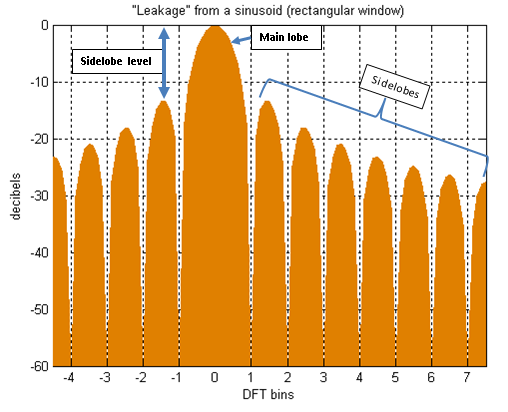
\includegraphics[scale=0.5]{cap4/spectleak}
    \caption{Spectral leakage}
    \label{spectleak}
  \end{center}
\end{figure}

Il calcolo del FFT su una finestra di osservazione non contenente un numero intero di periodi produce un allargamento e uno spostamento delle righe dello spettro di frequenza; questo fenomeno è chiamato \textit{spectral leakage} (dispersione spettrale, Figura \ref{spectleak}). 

Quindi, oltre a dover rispettare il teorema del campionamento di \textit{Nyquist}, bisogna prestare attenzione alla dispersione spettrale che causa \textit{aliasing} del segnale.

Applicare l'algoritmo di FFT direttamente alla sequenza campionata equivale ad usare una funzione di finestratura rettangolare, che pesa uniformemente i campioni.

Una soluzione che limita il fenomeno di \textit{spectral leakage} è l'utilizzo di una finestra rettangolare di troncamento contenente un numero intero di periodi. Tale soluzione non è sempre realizzabile perciò, nella pratica, si utilizza un'altra soluzione che consiste nel sostituire la finestra rettangolare con finestre che presentano una transizione graduale alle estremità. 

Pertanto, un importante aspetto da tenere in considerazione quando si esegue il calcolo della FFT di un segnale periodico campionato è l'operazione di finestratura \cite{31004}. 

Le finestre con transizione graduale alle estremità, chiamate anche \textit{smoothing window}, risolvono i problemi dovuti ad un campionamento non coerente. I problemi del campionamento non coerente si manifestano principalmente agli estremi della finestra di osservazione, dove si osservano discontinuità, quindi è ragionevole ipotizzare che se si potessero trascurare gli estremi e si potesse concentrare l'analisi sulla parte centrale della finestra di osservazione si otterrebbe uno spettro in frequenza più corretto. 

Pertanto, come già accennato, le \textit{smoothing window} pesano differentemente i vari campioni assumendo valore basso agli estremi e valore elevato nelle porzioni centrali della finestra.

Le \textit{smoothing window} sono divise tra finestre cosinusoidali e non cosinusoidali. Una delle più utilizzate è quella cosinusoidale di \textit{Hanning}.
\begin{figure}  
  \begin{center}
    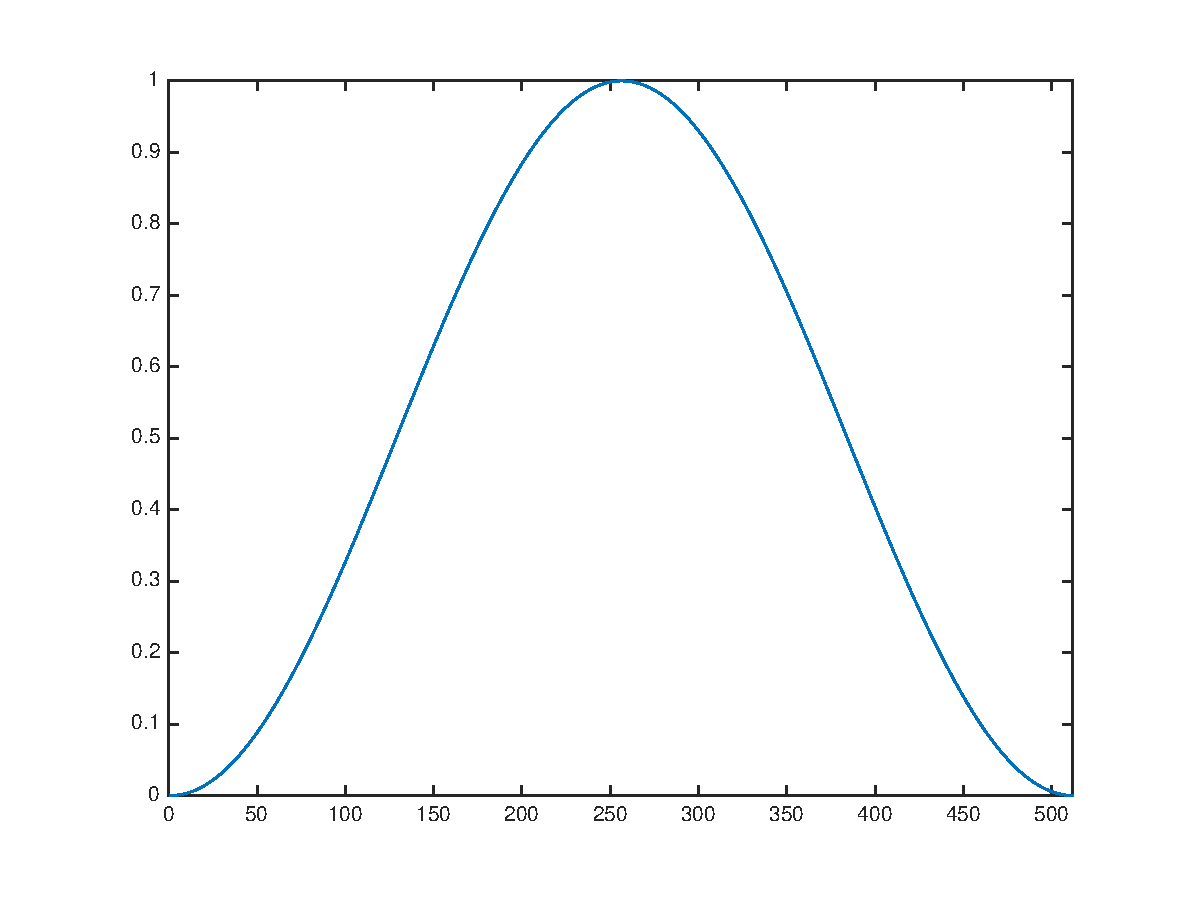
\includegraphics[scale=0.4]{cap4/hann}
    \caption{Finestra di Hanning}
    \label{hann}
  \end{center}
\end{figure}

La funzione peso della finestratura di \textit{Hanning} è definita dalla seguente relazione:
\begin{equation}
	w(n) = \frac{1}{2} \left [  1 - \cos \left ( \frac{2 \pi n}{N - 1} \right ) \right ]
\end{equation}
con:
$$ 0 \leq n \leq N-1 $$
ed è mostrata in figura \ref{hann}. La forma di questa finestra consente di eliminare la discontinuità del segnale agli estremi in caso di campionamento non coerente. 
\begin{figure}  
  \begin{center}
    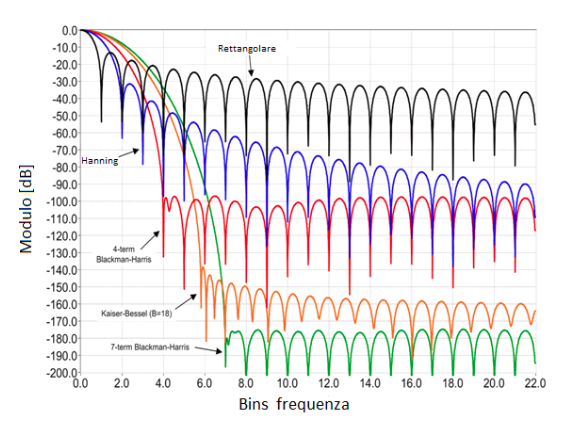
\includegraphics[scale=0.4]{cap4/smoothwins}
    \caption{Spectral leakage per diversi tipi di finestratura}
    \label{smoothwins}
  \end{center}
\end{figure}

Prima di eseguire l'algoritmo di FFT, quindi, ciascun campione della sequenza $x(n)$ viene moltiplicato per un coefficiente della funzione peso $w(n)$ della finestra. 
In figura \ref{smoothwins} è mostrato il confronto dello \textit{spectral leakage} per diversi tipi di finestratura. Emerge in modo chiaro dalla figura che l'utilizzo di \textit{smoothing window} riduce notevolmente il fenomeno di dispersione spettrale.

Concludendo, il parallelismo hardware intrinseco che si ottiene con l'FPGA è l'ideale per l'elaborazione numerica dei segnali in parallelo. Per tale motivo si è scelto di eseguire l'algoritmo di FFT su FPGA.

\subsection{Interpolated Fast Fourier Transform (IFFT)}
Come ampiamente descritto nel paragrafo precedente, per mezzo dell'algoritmo di FFT è possibile ricavare lo spettro di frequenza di un segnale. Lo spettro di frequenza ricavato è però discreto, pertanto le frequenze delle singoli componenti spettrali possono essere valutate dalla loro posizione nella spettro discreto con una risoluzione che dipende dal numero dei campioni \cite{31004}.

Se si campiona il segnale di ingresso con una frequenza $f_s$, si ottiene una risoluzione pari a:
\begin{equation}
	\Delta f = \frac{f_s}{N}
	\label{deltaf}
\end{equation}
dove $N$ è il numero dei campioni e $\Delta f$ è la distanza tra 2 \textit{bin} consecutivi.

Per migliorare la risoluzione del tono principale del segnale esistono algoritmi che utilizzano metodi di interpolazione.
\begin{figure}  
  \begin{center}
    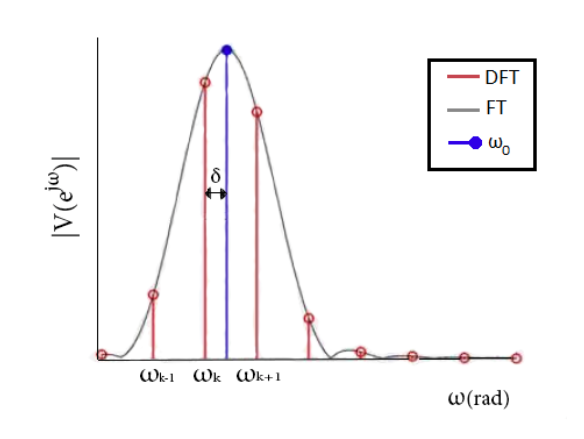
\includegraphics[scale=0.4]{cap4/ifft}
    \caption{Confronto tra DFT e FT di un segnale a frequenza $\omega _0$}
    \label{ifft}
  \end{center}
\end{figure}

Questi algoritmi, chiamati \textit{Interpolated FFT (IFTT) algorithm}, permettono di trovare la correzione di frequenza delta intorno alla frequenza del tono fondamentale allo scopo di ottenere la frequenza del segnale $\omega _0$  in modo più preciso:	
\begin{equation}
	\omega _0 = (k \pm \delta)\frac{2 \pi f_s}{N}
\end{equation}
con:
$$ 0 < \delta \leq 0.5$$
Gli algoritmi di interpolazione si dividono tra metodi a 2 punti e a 3 punti. Si è scelto di utilizzare algoritmi a due punti perchè essi limitano il contributo di rumore rispetto al caso a 3 punti. 

Per migliorare ulteriormente l'accuratezza dell'estrazione del tono è stato necessario utilizzare un algoritmo di interpolazione dei moduli specifico per segnali a cui è stata applicata la finestra di \textit{Hanning} \cite{1007077}. Pertanto, si mostra ora il procedimento per il calcolo del fattore di correzione $\delta$ nel caso di finestra di \textit{Hanning}.

Si consideri un segnale sinusoidale di frequenza $f_0$ campionato con periodo $T_s=\frac{1}{f_s}$:
\begin{equation}
	x(nT_s)=A_0 \sin ( 2 \pi f_0 n T_s + \phi ) \qquad n=0,1,...,N-1
	\label{xcampionato}
\end{equation}

Considerando la risoluzione $\Delta f $ dell'equazione \ref{deltaf}, possiamo riscrivere il tono fondamentale del segnale in funzione della dimensione del singolo \textit{bin}:
\begin{equation}
	f_0 = (L+\delta)\Delta f = \gamma \Delta f
\end{equation}
dove $L$ indica la parte intera di $\gamma$ e $\delta$ la correzione frazionaria di frequenza. Perciò, l'equazione \ref{xcampionato} si può riscrivere come:
\begin{equation}
	x[n]=A_0 \sin ( 2 \pi \gamma \frac{n}{N} + \phi ) \qquad n=0,1,...,N-1
\end{equation}
La DFT dell'equazione precedente alla linea spettrale $k$ è espressa dalla relazione:
\begin{equation}
	x[k] = \frac{1}{2} \left \{ A_0 e^{j\phi} W[(\gamma -k)f_0] + A_0 e^{-j\phi}W[(\gamma + k)f_0]  \right \}
\end{equation}
dove $W(f)$ è lo spettro di frequenza della funzione di finestratura utilizzata.

Come anticipato, la finestratura utilizzata è quella di \textit{Hanning} definita nel tempo come:	
\begin{equation}
w_{n,H}
\left\{\begin{matrix}
0.5 - 0.5\cos \left ( \frac{2 \pi}{N}n \right ) & & 0 \leq n \leq N \\ 
 0  &  & 0 > n \geq N
\end{matrix}\right.
\end{equation}
Lo spettro della finestra di \textit{Hanning} è espresso dalla relazione:
\begin{equation}
	W_H(f) = \frac{1}{2} \left \{ W_R (f) - \frac{1}{2} \left [ W_R (f+f_0) + W_R (f-f_0) \right ] \right \}
\end{equation}
dove $W_R (f)$ è lo spettro di frequenza della finestra rettangolare:
\begin{equation}
	W_R (f) = \frac{ \sin \left ( \pi \frac{f}{\Delta f} \right ) }{ \sin \left ( \pi \frac{f}{N \Delta f} \right ) } e^ { j \pi \frac{(N-1) f}{N \Delta f} }
\end{equation}

Considerando ora il calcolo della FFT sul segnale a cui è stata applicata la finestra di \textit{Hanning}: il risultato è la sequenza $X_h(n)$.

Determinato lo spettro $X_h(n)$, l'elaborazione continua calcolandone il modulo. \'E sufficiente calcolare il modulo di solo una metà della sequenza $X_h(n)$, poiché l'altra parte non aggiunge informazioni ulteriori.

Successivamente, si esegue la ricerca del valore massimo presente nel vettore $|X_h(n)|$ dei moduli calcolato al passo precedente: una volta individuato, si memorizza tale valore e la relativa posizione all'interno del vettore.

Se ipotizziamo che il bin di ampiezza maggiore sia $|X_h(k)|=|V_k|$ con $k$ posizione relativa al valore massimo presente nel vettore, mentre $|X_h(k+1)|=|V_{k+1}|$ sia quello con la seconda ampiezza più grande, possiamo stimare la correzione frazionaria  con la formula:
\begin{equation}
	\delta = \frac{2 |V_{k+1}|- |V_k|}{|V_{k+1}| + |V_k|}
\end{equation}

Per i passi che hanno portato alla stima della correzione $\delta$ si rimanda alla letteratura \cite{1007077}.

Le finestre utilizzate nel lavoro di tesi sono quella di \textit{Hanning} e quella rettangolare. Per tale motivo di seguito viene mostrato il fattore di correzione nel caso di finestra rettangolare.

Nel tempo la funzione che rappresenta la finestra rettangolare è definita con la relazione: 
\begin{equation}
w_{n,R}
\left\{\begin{matrix}
1 & & 0 \leq n \leq N \\ 
0  &  & 0 > n \geq N
\end{matrix}\right.
\end{equation}
e il fattore correttivo di frequenza $\delta$ è pari a:
\begin{equation}
	\delta = \frac{|V_{k+1}|}{|V_{k+1}| + |V_k|}
\end{equation}

Infine, per calcolare la frequenza del tono fondamentale è sufficiente usare la relazione: 
\begin{equation}
	f_0 = (k + \delta)\Delta f
\end{equation}

In questo modo, il valore del tono estratto viene scorrelato dalla larghezza del singolo \textit{bin}, riducendo notevolmente la risoluzione in frequenza. 

\subsection{Calcolo della distanza assoluta}
Come descritto in precedenza nel Capitolo \ref{capitolo2}, la distanza assoluta $s$ del bersaglio si ricava con la relazione:
\begin{equation}
	s = \frac{f_{rise}+f_{fall}}{2} \left [ \frac{\lambda^2}{2\left ( \frac{\Delta I}{\Delta T} \frac{\Delta \lambda}{\Delta I} \right )}  \right ]
\end{equation}
dove $f_{rise}$ e $f_{fall}$ sono rispettivamente il tono fondamentale del segnale interferometrico nella rampa di salita e discesa dell'onda triangolare.
	
\section{Architettura Software}
L'obiettivo principale del lavoro di tesi è lo sviluppo di un firmware, per la scheda di prototipazione, che sia in grado di computare e mostrare all'utente finale le misure di distanza assoluta prodotte da un laser mediante la tecnica di interferometria a retroiniezione.
\begin{figure}  
  \begin{center}
    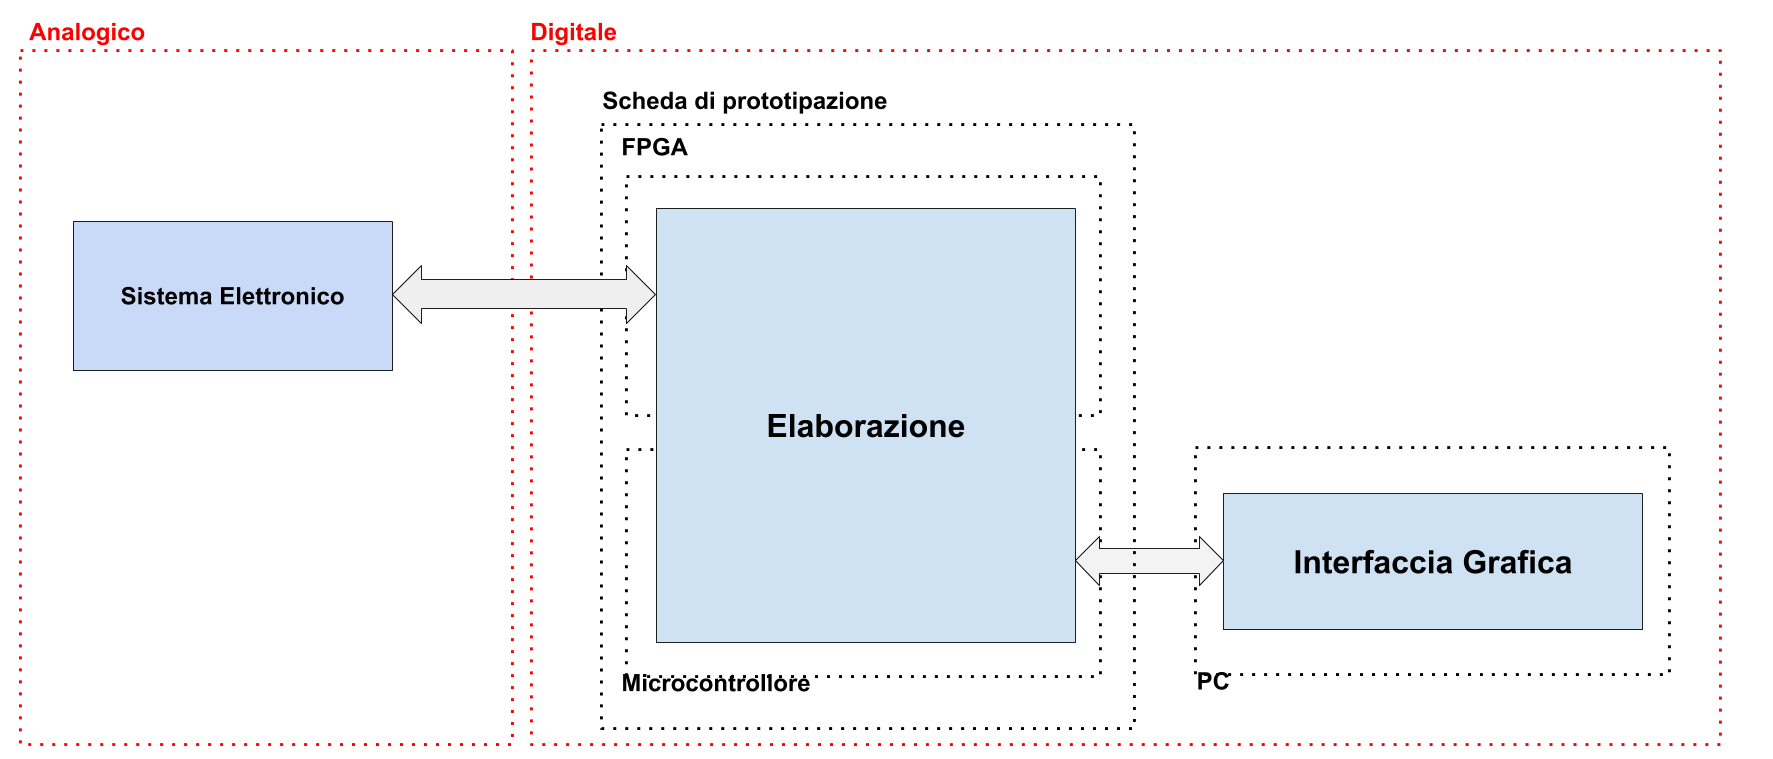
\includegraphics[scale=0.2]{cap4/archgenschema}
    \caption{Schema a blocchi ad alto livello dell'architettura}
    \label{archgenschema}
  \end{center}
\end{figure}

La computazione è completamente svolta sulla scheda di prototipazione, in parte su FPGA ed in parte su microprocessore. Mentre, è presente un computer connesso alla scheda che ha come unico scopo quello di mostrare i risultati dell'elaborazione mediante un interfaccia grafica. In figura \ref{archgenschema} è mostrato uno schema a blocchi ad alto livello dell'architettura appena descritta.

In particolare, l'elaborazione consiste, inizialmente, nell'acquisizione del segnale interferometrico in arrivo dal sistema elettronico del laser. Una volta acquisito, il segnale interferometrico viene condizionato e se ne estrae il tono fondamentale sfruttando l'algoritmo di FFT. Infine, utilizzando l'informazione del tono fondamentale del segnale, si ricava la misura di distanza assoluta che viene poi mostrata all'utente finale mediante l'interfaccia grafica.

Nei paragrafi successivi verranno descritte dettagliatamente le funzionalità svolte dall'FPGA e dal microcontrollore e come esse sono implementate via software.

\subsection{FPGA}
Le funzionalità svolte in hardware dal FPGA sono:
\begin{itemize}
	\item Generazione dei segnali di clock per la scheda di conversione
	\item Generazione del segnale di modulazione
	\item Campionamento del segnale interferometrico
	\item Condizionamento del segnale interferometrico
	\item Calcolo della Fast Fourier Transform (FFT)
	\item Estrazione del massimo bin di frequenza
\end{itemize}

\paragraph{Generazione dei segnali di clock per la scheda di conversione}
La scheda di conversione \textit{SCO Board} collegata ai pin digitali della board di prototipazione possiede due canali di conversione: un canale di conversione Analogico/Digitale collegato ai pin digitali d'ingresso e uno di conversione Digitale/Analogico collegato ai pin digitali d'uscita della \textit{sbRIO}. Entrambi i canali di conversione per funzionare correttamente vengono politati, dall'FPGA, con un segnale di clock a una frequenza di $30MHz$. Per garantire la sincronizzazione dei due canali di conversione viene utilizzato lo stesso segnale di clock per entrambi i circuiti di conversione.

\paragraph{Generazione del segnale di modulazione}
Il segnale di modulazione del laser viene generato, dai $12$ pin digitali d'uscita, sul fronte di salita del segnale di clock. Il segnale in uscita, generato punto per punto ad ogni ciclo di clock, è composto da $1250$ punti. Ogni punto è un dato binario da $12$ bit con una dinamica da $0$ a $4095$ livelli di tensione.

Il segnale di modulazione viene riprodotto completamente in uscita ogni $1250$ punti; questo fa si che il laser venga pilotato da un segnale di modulazione con frequenza pari a:
\begin{equation}
	f_{mod} = \frac{30MHz}{1250} = 24KHz
\end{equation}

\paragraph{Campionamento del segnale interferometrico}
Il segnale interferometrico in arrivo dal laser viene campionato, dai pin digitali d'ingresso, con una frequenza pari alla frequenza di clock ($30MHz$) e una risoluzione di $12$ bit.

Il segnale d'ingresso è anch'esso composto da $1250$ punti ognuno con una dinamica da $0$ a $4095$ livelli di tensione. Pertanto un segnale interferometrico completo equivalente a un periodo di modulazione del laser è disponibile ogni $41.6us$ ($24KHz$).

\paragraph{Condizionamento del segnale interferometrico}
Il segnale interferometrico, acquisito dal circuito di conversione Analogico/Digitale, viene condizionato prima di passato alla fase di elaborazione vera e propria.

Le operazione svolte nella fase di condizionamento sono:
\begin{itemize}
	\item Sottrazione del residuo
	\item Estrazione di 512 campioni
	\item Finestratura
\end{itemize}

\subparagraph{Sottrazione del residuo}
La sottrazione del residuo è un operazione che consiste nel sottrarre punto per punto al segnale interferometrico completo un segnale di $1250$ punti chiamato \textit{residuo}. Il \textit{residuo} è un segnale che viene calcolato e conservato nel FPGA nelle fasi preliminari di avviamento dello strumento di misura, il significato di tale segnale verrà illustrato nel Capitolo \ref{capitolo5}.

\subparagraph{Estrazione di 512 campioni}
Il segnale interferometrico, dopo essere stato privato del suo residuo, viene suddiviso in $2$ semiperiodi da $625$ campioni. Per ciascuno dei due semiperiodi vengono estratti solamente $512$ campioni contigui. I restanti $113$ campioni vengono scartati. 

Il motivo che ha spinto all'estrazione di soli $512$ campioni è dovuto all'algoritmo di FFT. Come spiegato in precedenza, tale algoritmo raggiunge ottime prestazioni con segnali che hanno lunghezza pari a una potenza di 2.

\subparagraph{Finestratura}
Ciascuno dei due sottoinsiemi da $512$ campioni viene poi moltiplicato punto per punto per una funzione finestra da $512$ punti a scelta tra quella rettangolare e quella di Hanning. La funzione finestra da utilizzare viene configurata in fase di inizializzazione dello strumento.

\paragraph{Calcolo della Fast Fourier Transform (FFT)}
La penultima funzionalità eseguita dal FPGA è il calcolo della Trasformata Discreta di Fourier (DFT) mediante l'algoritmo di FFT.

Il calcolo dell'FFT viene eseguito su ciascuno dei 2 sottoinsiemi da $512$ punti producendo in uscita, per ciascuno dei due sottoinsiemi, lo spettro di frequenza. In particolare, il risultato dell'algoritmo di FFT è composto da due array di $512$ punti contenenti rispettivamente la parte reale e immaginaria dello spettro di potenza del segnale nel dominio del tempo.

Dalla parte reale e immaginaria si ricava solamente, per ragioni dipendenti dalle performance del FPGA, il modulo quadrato dello spettro di frequenza.

Dato che i campioni in ingresso all'algoritmo di FFT sono campionati a $30MHz$, la risoluzione di frequenza di ciascun \textit{bin} è pari a:
\begin{equation}
	f_{bin} = \frac{f_{sample}}{n_{sample}} = \frac{30MHz}{512} = 58.59375 KHz
\end{equation}
Ciò significa che ciascun \textit{bin} di frequenza rappresenta la quantità totale di energia al quadrato posseduta dal segnale a quella particolare frequenza. Il primo punto corrisponde a $0Hz$ (componente continua), il secondo punto corrisponde a $58.59375 KHz$, il terzo punto corrisponde a $117.1875KHz$ e così via.

Sappiamo dal teorema di \textit{Nyquist} che il campionamento a $30MS/s$ sarà in grado di misurare frequenze fino a un massimo di $15MHz$. Perciò, tutti i bin maggiori al $257\degree$ (pari alla frequenza $256 * 58.59375 KHz = 15MHz$) rappresentano frequenze negative: il $258\degree$ corrisponde alla frequenza $-14.9414062 MHz$, il $259\degree$ corrisponde a $-14.8828124 MHz$ e così via.

\paragraph{Estrazione del massimo bin di frequenza}
L'ultima fase dell'elaborazione numerica del segnale interferometrico su FPGA è l'estrazione del bin di frequenza con massima ampiezza.

L'algoritmo per l'estrazione del massimo bin viene applicato solo su una parte dei $512$ bin di frequenza, questo perché il segnale interferometrico è un segnale puramente reale che non ha componenti immaginarie, e pertanto produce un FFT che è simmetrica rispetto alla componente continua $0 Hz$. Ciò significa che i valori a frequenze negative sono esattamente gli stessi delle loro controparti positive, e di conseguenza questi punti vengono considerati ridondanti e quindi scartati.

Inoltre, eliminando i primi campioni dello spettro si filtra la potenza della continua, poiché altrimenti risulterebbe il tono più alto. 

A questo punto, l'algoritmo di estrazione del massimo bin valuta il campione con ampiezza maggiore, corrispondente al tono fondamentale, ed estrae la sua posizione e la sua ampiezza, l'ampiezza del tono successivo e quella del tono precedente.

L'algoritmo effettua l'estrazione del massimo bin dopo ogni semiperiodo del segnale di modulazione. Ciò indica che la frequenza con cui viene prodotto un risultato è $48KHz$.

Infine, i risultati dell'elaborazione vengono inviati al microprocessore.

\subsubsection{Implementazione software}
Il software eseguito dall'FPGA è implementato su un unico VI, come richiesto da LabVIEW; infatti, a differenza di PC e microcontrollori, una FPGA che esegue codice LabVIEW può avere un solo VI in esecuzione simultanea.

Il VI sviluppato si compone di una \textit{Sequence Structure}, composta da 2 frame. La \textit{Sequence Structure} è un costrutto di LabVIEW utilizzato per imporre vincoli di precedenza temporale nell'esecuzione del codice. Questa scelta è stata fatta per garantire il corretto ordine di esecuzione delle istruzioni del codice, con il primo \textit{frame} che si occupa dell'inizializzazione dello strumento e il secondo e ultimo \textit{frame} che esegue le funzionalità precedentemente descritte.

Il \textit{frame} di inizializzazione si occupa di abilitare e inizializzare i pin digitali (DIO pin, \textit{Digital Input Output pin}) della scheda e di predisporre le memorie dell'FPGA per l'esecuzione. In particolare vengono inizializzate le memorie che conservano il segnale di modulazione, della funzione finestra e del residuo.

Il \textit{frame} finale è stato diviso in blocchi funzionali, ognuno contenente una porzione di funzionalità che è necessario garantire. I blocchi funzionali realizzati sono descritti di seguito:
\begin{itemize}
	\item \underline{Generazione del clock}, del \underline{segnale di modulazione} e \underline{acquisizione} del \underline{segnale interferometrico}: In questo blocco funzionale è implementata una macchina a stati finiti, composta da due stati: il primo attiva alto il segnale di clock per i circuiti di conversione DAC e ADC ed invia ai pin digitali di uscita il valore del punto del segnale di modulazione da generare. Nel secondo stato, invece, il segnale di clock per i circuiti di conversione viene portato basso e si legge il valore digitale presente ai pin d'ingresso della scheda che corrisponde al valore letto dal circuito elettronico del laser in quell'istante. In questo modo viene garantita una sincronizzazione tra il valore di modulazione e il valore di risposta del laser.
	\item \underline{Lettura dalla memoria del segnale di modulazione}: Questo blocco funzionale provvede a leggere dalla memoria, precedentemente inizializzata, il punto successivo del segnale di modulazione usato per pilotare il laser. Ogni punto letto viene inviato al blocco di generazione del segnale di modulazione.
	\item \underline{Condizionamento del segnale}: Questo blocco funzionale riceve il segnale dal blocco di acquisizione e esegue le operazioni di condizionamento. Infine, invia il segnale condizionato, punto per punto, al blocco di computazione dell'FFT.
	\item \underline{Computazione FFT}: In questo blocco si esegue l'algoritmo di FFT sulla porzione di segnale precedentemente condizionata. L'algoritmo di FFT viene eseguito in pipeline con una latenza di $1316$ cicli di clock. Il risultato dell'algoritmo viene inviato, punto per punto, al blocco finale.
	\item \underline{Calcolo del massimo bin dell'FFT}: Per ogni risultato generato dal blocco di computazione dell'FFT si verifica se quest'ultimo è quello di ampiezza massima finora rilevato e si provvede a salvare in dei registri il numero del bin con la relativa ampiezza, oltre all'ampiezza precedente e successiva. Questi valori vengono poi inviati al microprocessore per poter eseguire l'FFT interpolata e ricavare il tono fondamentale dal segnale.
\end{itemize}

Ogni blocco funzionale è rappresentato graficamente da un ciclo. I cicli vengono eseguiti fisicamente in parallelo, per via delle caratteristiche intrinseche dell'esecuzione su FPGA, e la comunicazione inter-processo avviene utilizzando delle code dati chiamate \textit{FIFO}. 
\begin{figure}  
  \begin{center}
    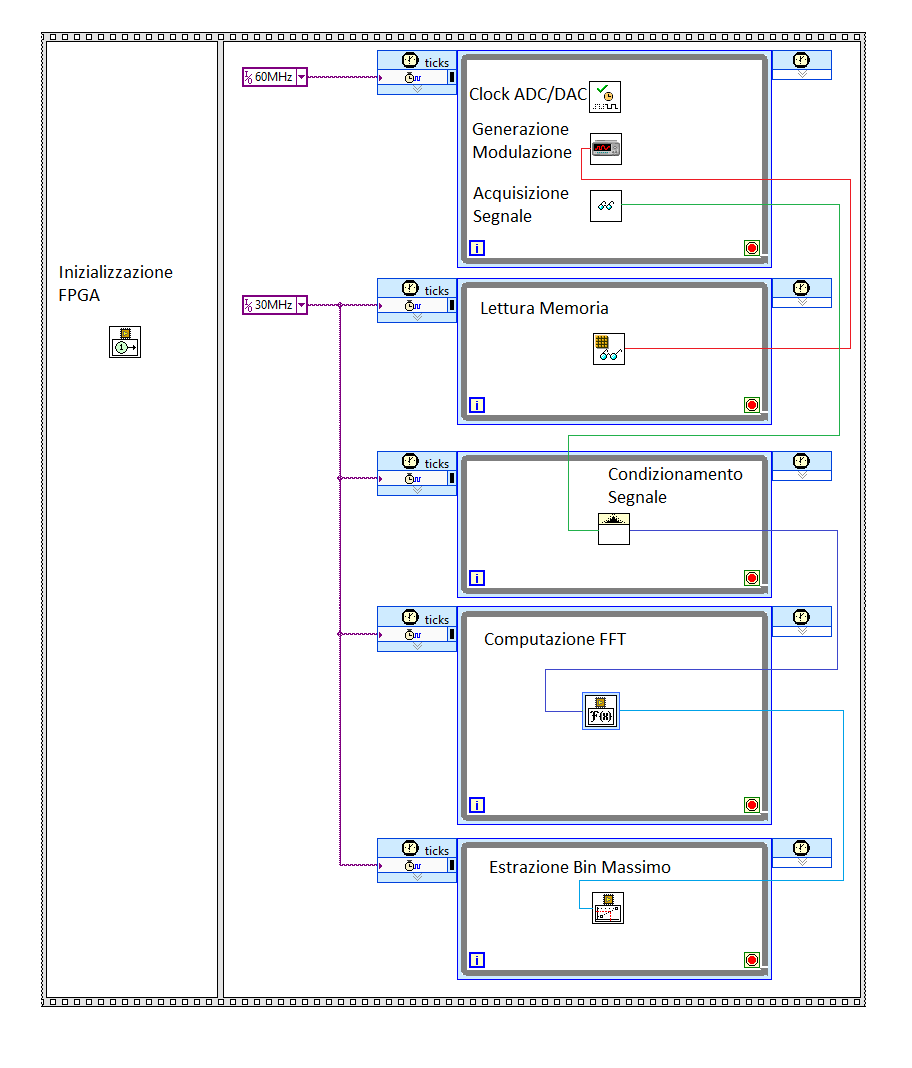
\includegraphics[scale=0.5]{cap4/codicefpga}
    \caption{Block Diagram semplificato del VI eseguito su FPGA}
    \label{codicefpga}
  \end{center}
\end{figure}

In Figura \ref{codicefpga} è mostrata una versione semplificata del diagramma a blocchi utilizzato per implementare le funzionalità FPGA soprascritte. Il primo ciclo possiede una frequenza di $60MHz$ per garantire la corretta generazione del clock a $30MHz$ per i circuiti di conversione A/D e D/A, al contrario dei restanti cicli che hanno frequenza $30MHz$.
	
\paragraph{Design pattern utilizzati}
Nello sviluppo del codice eseguito in hardware dall'FPGA ci si è serviti di due \textit{design pattern} tipicamente utilizzati durante lo sviluppo di codice LabVIEW: il \textit{Producer-Consumer} e il \textit{4-Wire Handshake}, che verranno spiegati in dettaglio nel seguito del paragrafo.

\subparagraph{Producer-consumer}
Il \textit{Producer-Consumer design pattern} è un pattern utilizzato per la sincronizzazione tra processi basato sul Master/Slave pattern. Il problema descrive due processi, uno produttore (\textit{Producer, Master}) ed uno consumatore (\textit{Consumer, Slave}), che condividono una memoria comune, chiamata buffer, di dimensione fissata. 

Il compito del produttore è generare dati e depositarli nel buffer. Contemporaneamente, il consumatore utilizzerà i dati prodotti, rimuovendoli di volta in volta dal buffer. Il problema è assicurare che il produttore non elabori nuovi dati se il buffer è pieno, e che il consumatore non cerchi dati se il buffer è vuoto.

In LabVIEW i processi producer e consumer sono rappresentati rispettivamente da due cicli (\textit{While} o \textit{Timed-Loop}) eseguiti in parallelo, mentre il buffer è rappresentato da una memoria \textit{FIFO}. 
\begin{figure}  
  \begin{center}
    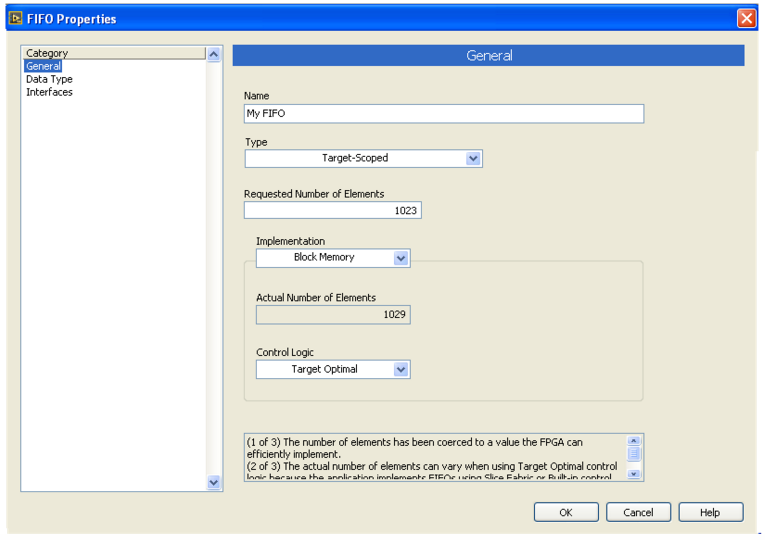
\includegraphics[scale=0.4]{cap4/fifolabview}
    \caption{Pannello di configurazione per la creazione di una FIFO}
    \label{fifolabview}
  \end{center}
\end{figure}

La \textit{FIFO} è una struttura dati che contiene gli elementi nell'ordine in cui sono ricevuti e fornisce l'accesso a quest'ultimi usando un criterio \textit{First-In First-Out}. Quando si configura una FIFO, è necessario specificarne la dimensione e la tipologia di dato (Figura \ref{fifolabview}).
\begin{figure}  
  \begin{center}
    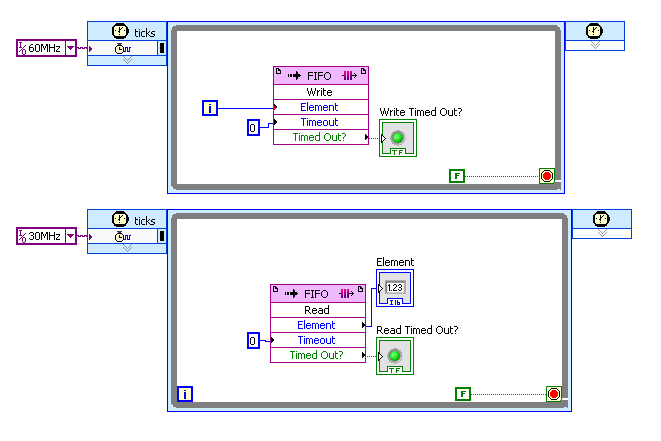
\includegraphics[scale=0.5]{cap4/prodcons}
    \caption{Esempio di Producer/Consumer implementato su LabVIEW FPGA}
    \label{prodcons}
  \end{center}
\end{figure}

La Figura \ref{prodcons} seguente mostra un esempio in LabVIEW di Producer/Consumer pattern utilizzato per trasferire dati tra due cicli Single Timed Loop sulla stessa FPGA. I due processi risiedono su due diversi domini di frequenza: il producer utilizza un clock a $60 MHz$ mentre il consumer utilizza un clock a $30 MHz$. 

Nel processo producer, le letture relative al numero dell'iterazione del ciclo vengono scritte nel buffer di memoria FIFO attraverso il nodo \textit{FIFO Method Node Write}. Se il dato numerico in ingresso al metodo non è disponibile o la coda è piena, il metodo \textit{Write} non scrive alcun dato nella coda e asserisce l'uscita \textit{Timed Out?} a vero segnalando che l'elemento non è stato depositato nella coda. Il metodo \textit{FIFO Method Node Read}, nel processo consumer, legge i dati dalla coda. Se i dati non sono disponibili per la lettura asserisce l'uscita \textit{Timed Out?} a vero segnalando che la coda è vuota.

\subparagraph{4-Wire Handshake}
L'implementazione \textit{pipelined} dell'\textit{express VI} FFT ha richiesto l'uso del pattern del \textit{4-wire handshake} \cite{4wirehs}.

Il \textit{4-wire handshake} è un pattern tipicamente usato nell'implementazione di sub-VI eseguiti in pipeline nell'ambito di LabVIEW FPGA.

Nei nodi che consentono l'utilizzo di questo pattern tipicamente si hanno due ingressi e due uscite aggiuntive, che consentono l'implementazione del protocollo:
\begin{itemize}
	\item \underline{Ingressi}
	\begin{itemize}
	\item \textit{Input Valid}: specifica che il prossimo dato da processare è pronto in ingresso
	\item \textit{Ready for output}: Specifica se i nodi a valle sono pronti per ricevere nuovi dati in ingresso
	\end{itemize}
	\item \underline{Uscite}
	\begin{itemize}
	\item \textit{Output valid}: specifica ai nodi a valle che il dato corrente in uscita è valido
	\item \textit{Ready for input}: specifica se il subVI può ricevere nuovi dati in ingresso al prossimo ciclo
	\end{itemize}
\end{itemize}

\begin{figure}  
  \begin{center}
    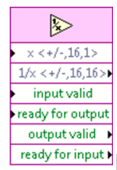
\includegraphics[scale=0.4]{cap4/pipelinevi}
    \caption{Ingressi ed uscite di un express VI con esecuzione pipelined}
    \label{pipelinevi}
  \end{center}
\end{figure}

L'esecuzione del protocollo \textit{4-Wire Handshake} inizia con il nodo pipelined che comunica alla coda in ingresso che è pronto per accettare nuovi dati in ingresso. Tipicamente è utilizzato un feedback node per comunicare il valore logico della variabile \textit{ready for input} ai nodi a valle del subVI. 

Quando il nodo a valle del subVI fornisce il dato assegna il valore logico Vero alla variabile \textit{Input Valid} indicando così al subVI che il dato al suo ingresso è pronto per essere processato. Se il nodo pipelined ha ricevuto tutti i dati di cui necessitava il valore logico della variabile \textit{Ready for input} viene portato a Falso.

Al termine della computazione il subVI attende che il valore della variabile \textit{ready for output} sia Vero e modifica il valore logico della variabile \textit{output valid} a Vero, per comunicare ai nodi a monte che il valore in output è valido. Contemporaneamente il valore della variabile \textit{ready for input} viene portato a Vero, per poter accettare un nuovo valore in ingresso e ricominciare la computazione.

Nel caso del subVI dell'FFT il valore di \textit{input ready} è dato dal \textit{Time out?} della coda FIFO \textit{Waveform}; infatti, se la coda contiene almeno un dato al suo interno, il dato che fornisce è valido. Al termine della computazione dell'FFT il valore \textit{output valid} consente al calcolo del modulo al quadrato dell'FFT di essere eseguito, e, come specificato dal pattern, il valore logico di \textit{ready for input} viene portato a Vero.

Poiché il calcolo del modulo quadrato dell'FFT non è stato sviluppato sfruttando la pipeline, esso è sempre pronto a ricevere un input, rendendo il valore di \textit{ready for output} sempre Vero.

\begin{figure}  
  \begin{center}
    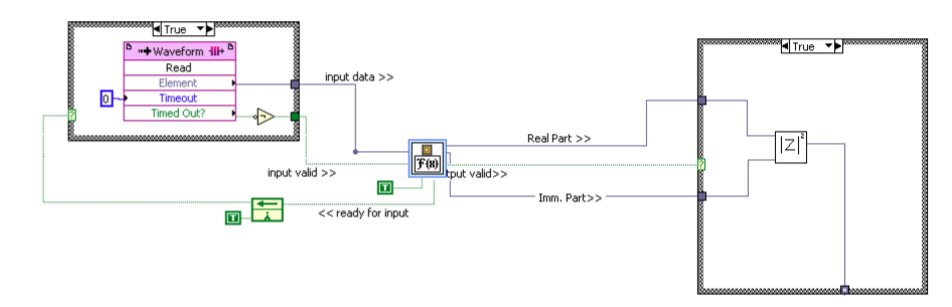
\includegraphics[scale=0.35]{cap4/fftloop}
    \caption{Computazione FFT}
  \end{center}
\end{figure}

\begin{figure}  
  \begin{center}
    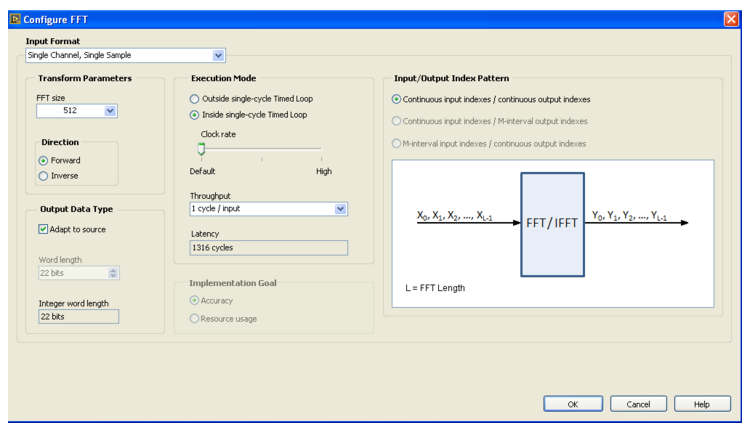
\includegraphics[scale=0.3]{cap4/configfft}
    \caption{Pannello di configurazione del FFT Express VI}
    \label{configfft}
  \end{center}
\end{figure}

Il SubVI \textit{FFT Express VI}, che effettua la computazione del FFT, è inserito all'interno di un \textit{Single Cycle Timed Loop}. Esso effettua il calcolo dell'FFT di $512$ campioni con una latenza di $1316$ cicli di clock ($\frac{1316}{30MHz}=43.86us$) e un \textit{throughput} di ingresso pari a $1\ input/ciclo$. In Figura \ref{configfft} è mostrato il pannello di configurazione dell'\textit{FFT Express VI}.

\begin{figure}  
  \begin{center}
    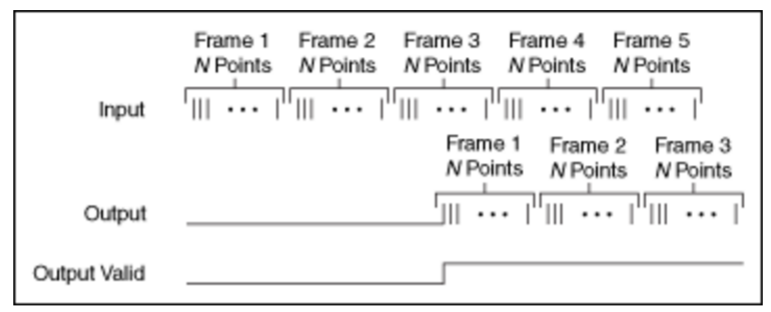
\includegraphics[scale=0.3]{cap4/timdiagfft}
    \caption{FFT Express VI Timing Diagram}
    \label{timdiagfft}
  \end{center}
\end{figure}

ll \textit{Timing diagram} in Figura \ref{timdiagfft} mostra le relazioni temporali tra gli ingressi e le uscite dell'FFT Express VI quando esso si trova all'interno di un single-cycle Timed Loop con Throughput pari 1 input/ciclo.

			
\paragraph{Fixed Point}
Per motivi di prestazioni e di area, è stato ampiamente utilizzato il tipo di dato \textit{fixed point} nello sviluppo del codice FPGA. Per i precedenti motivi, inoltre, le funzioni di libreria presenti in LabVIEW FPGA accettano come ingressi numeri rappresentati in \textit{fixed point}.
\begin{figure}  
  \begin{center}
    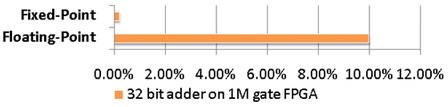
\includegraphics[scale=0.7]{cap4/fxpvsfloat}
    \caption{Confronto dello spazio occupato da un sommatore su FPGA con Fixed Point e Floating Point}
    \label{fxpvsfloat}
  \end{center}
\end{figure}

Come specificato dalla documentazione di LabVIEW \cite{fxpdoc}, l'utilizzo di algebra \textit{fixed point} permette di avere un risparmio notevole in termini di area utilizzata su FPGA rispetto all'uso del \textit{floating point}, come è visibile in Figura \ref{fxpvsfloat}.

Il tipo di dato \textit{fixed point} è caratterizzato da tre parametri: la lunghezza in numero di bit (\textit{word length}), la lunghezza della parte intera (\textit{integer word length}) e la presenza del segno (\textit{signed/unsigned}). Inoltre è possibile scegliere se implementare un ulteriore bit in grado di segnalare la presenza di overflow e di scegliere il comportamento in caso di overflow.

La lunghezza della parte intera può essere maggiore o minore rispetto alla lunghezza della parola. Nel primo caso non è possibile rappresentare numeri con una parte decimale, mentre nel secondo caso i numeri avranno una parte decimale con una lunghezza in bit pari alla differenza tra la lunghezza della parola e della parte intera. 

\'E anche possibile rappresentare numeri con parte intera negativa. In questo caso non è possibile rappresentare numeri interi, ed in particolare si potranno rappresentare soltanto numeri compresi tra $0$ e $1$ in caso di \textit{fixed point unsigned}, oppure tra $-1$ e $1$ in caso di \textit{fixed point signed}.

Per lo sviluppo del progetto sono stati utilizzati fixed point signed a $12$-bit con parola intera di $12$ bit per i segnali generati ed acquisiti. Questa scelta è stata fatta tenendo conto della risoluzione dei convertitori utilizzati, che è appunto di $12$-bit.

Per quanto riguarda le restanti configurazioni del tipo di dato all'interno del codice si è fatto affidamento al sistema di auto-adattamento delle uscite in base alla lunghezza dei risultati integrato in LabVIEW. Questo sistema calcola il massimo valore rappresentabile in uscita da un blocco funzionale e adatta il tipo di dato di conseguenza.

\begin{figure}  
  \begin{center}
    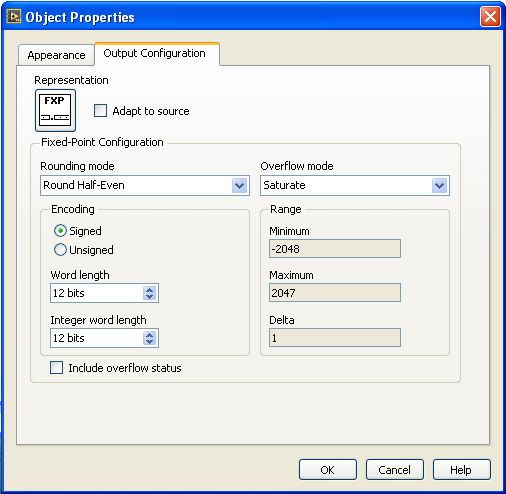
\includegraphics[scale=0.5]{cap4/configfxp}
    \caption{Fixed point in LabVIEW}
    \label{configfxp}
  \end{center}
\end{figure}

\subsection{Microcontrollore}
Il software sviluppato per l'esecuzione su microcontrollore svolge le funzionalità che, per via della struttura intrinseca e dei limiti di spazio dell'FPGA, non è stato possibile implementare direttamente in hardware. In particolare il software eseguito sul microcontrollore fornisce le seguenti funzionalità:
\begin{itemize}
	\item Algoritmo per il controllo del rumore
	\item Calcolo della Fast Fourier Transform interpolata (IFFT)
	\item Calcolo della frequenze di frangia
	\item Calcolo della distanza assoluta
\end{itemize}

\paragraph{Algoritmo per il controllo del rumore}
A causa di possibili disturbi esterni, non tutte le misure sono da ritenere valide. È stato quindi implementato un algoritmo di controllo che scartasse le ampiezze dei bin qualora fossero palesemente errate.

Per fare ciò si è usato un semplice criterio di selezione: se le ampiezze dei bin massimo e laterali sono al di sotto di una determinata soglia, chiamata "soglia di rumore", vengono scartate altrimenti accettate. Le ampiezze vengono accettate se e solo se tutte le ampiezze di un periodo di modulazione superano positivamente il criterio di selezione.

La "soglia di rumore" è la massima ampiezza raggiungibile da un bin di frequenza in assenza di ostacolo da misurare. Essa viene calcolata rimuovendo l'ostacolo e non considerando le ampiezze dei primi bin.

\paragraph{Calcolo della Fast Fourier Transform interpolata (IFFT)}
La funzionalità più importante eseguita dal microprocessore è il calcolo dell'FFT interpolata (IFFT). 

I dati, ricevuti del FPGA, relativi alle ampiezze dei bin massimo e laterali sono espressi come modulo al quadrato. Per permettere la corretta esecuzione dell'algoritmo di IFFT è necessario, però, che le ampiezze siano espresse in modulo, per questo motivo viene applicata l'operazione di radice quadrata per convertirli.
Ultimata l'operazione di radice quadrata, viene calcolato, per ogni FFT computata dal FPGA, il fattore di correzione della frequenza.

Se la funzione finestra utilizzata è la rettangolare viene applicata l'equazione:
\begin{equation}
	\delta = \frac{|V_{x}|}{|V_{k}|+|V_{x}|}
\end{equation}
dove:
\begin{itemize}
	\item $k$ è il bin di frequenza di ampiezza massima
	\item $|V_k|$ è il modulo del bin di ampiezza massima
	\item $|V_{k-1}|$ è il modulo del bin precedente al massimo
	\item $|V_{k+1}|$ è il modulo del bin successivo al massimo
	\item $|V_x|$ è il massimo tra $|V_{k-1}|$ e $|V_{k+1}|$ 
\end{itemize}

Altrimenti, se la funzione finestra utilizzata è \textit{Hanning} viene applicata l'equazione:
\begin{equation}
	\delta = \frac{2|V_{x}|-|V_{k}|}{|V_{k}|+|V_{x}|}
\end{equation}

Infine, la correzione di frequenza  viene aggiunta al massimo bin $k$ calcolato dal FPGA ottenendo così il bin interpolato:
\begin{equation}
	k'=k+\delta
\end{equation}
con $ 0 < \delta \leq 0.5 $.

\paragraph{Calcolo delle frequenze di frangia}
La frequenza del segnale, in funzione del bin interpolato, si calcola con la relazione:
\begin{equation}
	f_0 = \frac{f_{sample}}{N} k' = \frac{30MHz}{512} k'
\end{equation}
Per preparare il sistema ad eseguire la misura di distanza assoluta è necessario analizzare separatamente i dati corrispondenti al semiperiodo di discesa e al semiperiodo di salita del segnale triangolare di modulazione, in modo da estrarre separatamente i toni fondamentali $f_{fall}$ e $f_{rise}$.

\paragraph{Calcolo della distanza assoluta}
L'ultima operazione compiuta dal microcontrollore è il calcolo della distanza assoluta mediante la relazione:
\begin{equation}
	s = \frac{f_{rise}+f_{fall}}{2} \left [ \frac{\lambda^2}{2\left ( \frac{\Delta I}{\Delta T} \frac{\Delta \lambda}{\Delta I} \right )}  \right ] = \frac{f_{rise}+f_{fall}}{2} \Psi
\end{equation}

Il parametro $\Psi = \frac{\lambda^2}{2\left ( \frac{\Delta I}{\Delta T} \frac{\Delta \lambda}{\Delta I} \right )} $ non è definito, questo perché $\frac{\Delta \lambda}{\Delta I}$ non è noto a priori, ma si può ritenere in prima approssimazione costante, e si può ricavare variando la distanza e mantenendo tutti gli altri parametri costanti. Dopo aver mediato i risultati si ottiene $\Psi=261.5 nm/Hz$.

Inoltre, è possibile mediare $M$ misure di distanza ottenendo così una misura più accurata mediante la relazione:
\begin{equation}
	\bar{s} = \frac{\sum_{i=1}^{M} s_i}{M}
\end{equation}

L'introduzione del calcolo della media di $M$ distanze assolute riduce il \textit{throughput} di misura di un fattore $M$. 

\subsubsection{Implementazione software}
Il software sviluppato per essere eseguito su microcontrollore è contenuto in un unico VI, nonostante questo non sia un obbligo imposto dal linguaggio. La scelta di utilizzare un singolo VI è stata fatta per semplificare il processo di sviluppo; tuttavia sono stati sviluppati più VI, utilizzati poi come subVI nell'unico VI eseguito dal microcontrollore, per rendere il codice più leggibile e lo sviluppo più modulare.

Il VI principale eseguito dal microcontrollore si compone di una parte di codice sequenziale che svolge l'inizializzazione ed in seguito di due cicli paralleli, uno per leggere i dati inviati dall'FPGA ed uno per elaborare i dati ricevuti. La comunicazione tra i due cicli è fatta utilizzando il già descritto pattern del Producer-Consumer.

La parte di codice iniziale si occupa della configurazione dello strumento, inviando all'FPGA il \textit{bitfile} da eseguire, i parametri di esecuzione ed il contenuto delle memorie. Il ciclo di elaborazione, invece, esegue tutte le funzionalità appena descritte.

L'interfaccia grafica, che corrisponde al front panel del VI implementato su microcontrollore, viene eseguita su un PC collegato con cavo \textit{Ethernet} alla scheda di prototipazione. Il microcontrollore invia, attraverso il protocollo \textit{Ethernet}, i dati da visualizzare graficamente sugli indicatori del front panel.

\begin{figure}  
  \begin{center}
    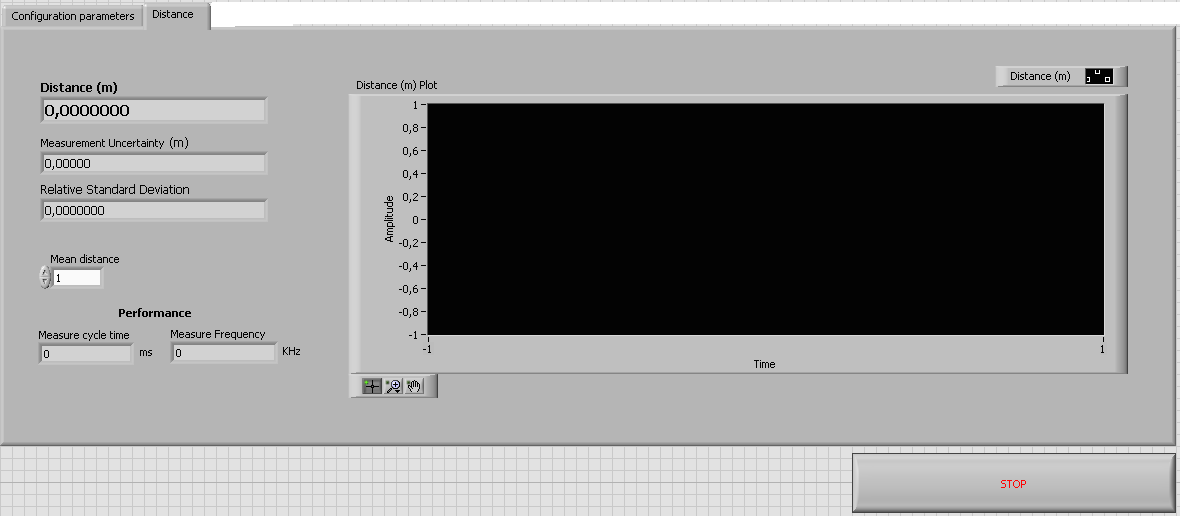
\includegraphics[scale=0.3]{cap4/guimicro}
    \caption{Interfaccia grafica dello strumento di misura}
    \label{guimicro}
  \end{center}
\end{figure} 

\subsection{Comunicazione tra FPGA e Microcontrollore}
Lo comunicazione tra il microprocessore e il chip FPGA avviene attraverso l'utilizzo di un componente hardware dedicato chiamato DMA.

Il DMA, acronimo di \textit{Direct Memory Access}, di una CPU è quel meccanismo che permette ad altri sottosistemi, quali ad in esempio le periferiche, di accedere direttamente alla memoria interna per scambiare dati, in lettura e/o scrittura, senza coinvolgere l'unità di controllo per ogni byte trasferito tramite l'usuale meccanismo dell'interrupt e la successiva richiesta dell'operazione desiderata, ma generando un singolo interrupt per blocco trasferito \cite{tanembaum}. Nella nostra architettura il sottosistema in questione è il chip FPGA.

L'utilizzo del DMA permette al chip FPGA di trasferire grosse quantità di dati sulla memoria del Real-Time host senza l'intervento del microprocessore. Questo meccanismo offre un notevole incremento delle prestazioni del sistema poiché il microprocessore, non essendo impegnato nel trasferimento dei dati, può svolgere altre operazioni.
\begin{figure}  
  \begin{center}
    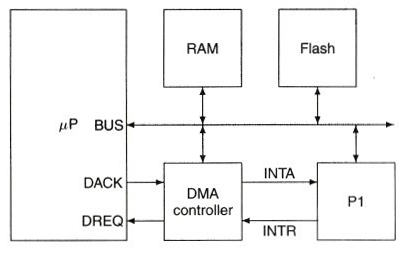
\includegraphics[scale=0.6]{cap4/dmafunz}
    \caption{Schema architetturale per DMA}
    \label{dmafunz}
  \end{center}
\end{figure} 

Di seguito è descritto il funzionamento generale di una DMA. Lo schema generale di funzionamento è mostrato in Figura \ref{dmafunz}.

Il flusso degli eventi che caratterizzano un trasferimento mediante DMA inizia con l'asserzione di un segnale di interrupt (INTR). Il DMA controller, dispositivo incaricato di interfacciarsi con microprocessore e periferiche, rileva la richiesta e richiede al microprocessore, con un segnale di interrupt (DREQ) il controllo del bus dati. Quando il microprocessore è pronto per rilasciare il bus dati lo segnala al DMA controller con un segnale di acknowledgement (DACK). Successivamente, il DMA controller, comunica alla periferica, mediante il segnale di INTA, che la trasmissione dei dati può avere inizio. Il DMA controller trasferisce i dati in arrivo dalla periferica sulla memoria senza l'intervento del microprocessore. Al termine della trasmissione, il DMA controller de-asserisce i segnali di DREQ e INTA e la periferica il segnale di INTER. A sua volta il microprocessore abbassa il segnale di DACK.

In LabVIEW FPGA questo flusso di eventi è nascosto al programmatore. L'ambiente di sviluppo mette a disposizione dei nodi \textit{Read DMA} e \textit{Write DMA} che svolgono al loro interno il protocollo di trasmissione appena descritto.

